\documentclass[10pt]{mybook4}
\pagestyle{myheadings}
\newcommand{\markchapter}[1]{\markboth{
   \mbox{}\hfill {\it Chapter \thechapter}. \ {\it #1}  \hfill  \mbox{}\hspace{-\textwidth} \protect\rule[-2mm]{\textwidth}{.15mm}}{}}

\newcommand{\markchapterapp}[1]{\markboth{
   \mbox{}\hfill \ {\it #1}  \hfill  \mbox{}\hspace{-\textwidth} \protect\rule[-2mm]{\textwidth}{.15mm}}{}}

\newcommand{\nomarkchapter}{\markboth{
\mbox{} \hfill  \mbox{}\hspace{-\textwidth}
\protect\rule[-2mm]{\textwidth}{.15mm}} {\protect\rule
[-2mm]{\textwidth}{.15mm} \hspace{-\textwidth}\mbox{} \hfill
\mbox{}}}
\newcommand{\markintro}{\markboth{
\mbox{}\hfill {\it Chapter \thechapter}. \ {\it Introduction}
\hfill  \mbox{}\hspace{-\textwidth}
\protect\rule[-2mm]{\textwidth}{.15mm}}{\protect\rule
[-2mm]{\textwidth}{.15mm}
     \hspace{-\textwidth}\mbox{} \hfill  {\it Chapter \thechapter}. \ {\it Introduction} \hfill \mbox{}}}
\newcommand{\marksam}[1]{\markboth{\mbox{}\hfill {\it Samenvatting} \hfill \mbox{} \hspace{-\textwidth} \protect\rule[-2mm]{\textwidth}{.15mm}}
{\protect\rule [-2mm]{\textwidth}{.15mm} \hspace{-\textwidth}\mbox{}
\hfill {\it Samenvatting} \hfill \mbox{}} }
\newcommand{\markref}{\markboth{
     \mbox{}\hfill {\it References} \hfill \mbox{}
     \hspace{-\textwidth} \protect\rule[-2mm]{\textwidth}{.15mm}}{\protect\rule [-2mm]{\textwidth}{.15mm}
     \hspace{-\textwidth}\mbox{} \hfill  {\it References} \hfill \mbox{}}}
\newcommand{\marksection}[1]{\markright{\protect\rule
     [-2mm]{\textwidth}{.15mm}
     \hspace{-\textwidth}\mbox{} \hfill  {\it \thesection} \ {\it #1} \hfill \mbox{}}}
\newcommand{\markcon}{\markboth{
    \mbox{}\hfill {\it Contents} \hfill \mbox{}
   \hspace{-\textwidth} \protect\rule[-2mm]{\textwidth}{.15mm}}{\protect\rule [-2mm]{\textwidth}{.15mm}
  \hspace{-\textwidth}\mbox{} \hfill  {\it Contents} \hfill \mbox{}}}
\newcommand{\markab}[1]{\markboth{
     \mbox{}\hfill List of Abbreviations \hfill \mbox{}
     \hspace{-\textwidth} \protect\rule[-2mm]{\textwidth}{.15mm}}{}}
\newcommand{\marklt}{\markboth{
     \mbox{}\hfill {\it List of Tables} \hfill \mbox{}
     \hspace{-\textwidth} \protect\rule[-2mm]{\textwidth}{.15mm}}{\protect\rule [-2mm]{\textwidth}{.15mm}
     \hspace{-\textwidth}\mbox{} \hfill  {\it List of Tables} \hfill \mbox{}}}
\newcommand{\marklf}{\markboth{
     \mbox{}\hfill {\it List of Figures} \hfill \mbox{}
     \hspace{-\textwidth} \protect\rule[-2mm]{\textwidth}{.15mm}}{\protect\rule [-2mm]{\textwidth}{.15mm}
     \hspace{-\textwidth}\mbox{} \hfill  {\it List of Figures} \hfill \mbox{}}}

\setlength{\evensidemargin}{1.46cm}
\setlength{\oddsidemargin}{1.46cm} \setlength{\topmargin}{2.31cm}
\setlength{\headheight}{4mm} \setlength{\headsep}{1.2cm}
\setlength{\textwidth}{13cm} \setlength{\textheight}{18.4cm}



\renewcommand{\baselinestretch}{1.25}
\renewcommand{\arraystretch}{1}
\setlength{\arrayrulewidth}{0.75pt}
\renewcommand{\thefootnote}{\fnsymbol{footnote}}



%new settings
%\setlength{\pagewidth}{17cm}
%\setlength{\pageheight}{24cm}
\setlength{\evensidemargin}{1.46cm}
\setlength{\oddsidemargin}{1.46cm} \setlength{\topmargin}{2.31cm}
\setlength{\headheight}{4mm} \setlength{\headsep}{1.2cm}
\setlength{\textwidth}{13cm} \setlength{\textheight}{18.4cm}

\renewcommand{\baselinestretch}{1.25}
\renewcommand{\arraystretch}{1}
\setlength{\arrayrulewidth}{0.75pt}
\renewcommand{\thefootnote}{\fnsymbol{footnote}}

\usepackage{graphicx,epsfig,fancybox,lscape}
\usepackage{latexsym,psfig,amssymb, amsmath}
\usepackage{subfigure}

\usepackage{natbib}
\usepackage[dvips]{color}
\usepackage{shadow}
%\usepackage{pstcol,pst-grad}
\usepackage{graphics}
\usepackage{amsmath,amsfonts}
\usepackage{pstricks}
\usepackage{float}
\usepackage{multirow}
\usepackage{amssymb}
\usepackage{multirow}
\usepackage{rotating}
\usepackage{sweave}
\usepackage{bm}

%%%%%%%%%%%%


%%%%%%%%%%%%

\newtheorem{thm}{Theorem}[section]
\newtheorem{lem}[thm]{Lemma}
\newenvironment{dfn}{\refstepcounter{thm} \bigskip \par \noindent
    {\bf Definition \thethm}\ }{\bigskip \par}


% FOI23a.TEX
% begin preamble
%
%\documentclass{statsoc}
%\usepackage{verbatim}
%\input table
%\newcommand{\dir}{c:/marc.ziv/sambvd}
%\newcommand{\chs}[2]{\mbox{$\left(
%\begin{array}{c}
%#1\\#2
%\end{array}
%\right)
%$}}

%\newcommand{\trialr}{\mbox{\tiny trial(r)}}
%\newcommand{\trialf}{\mbox{\tiny trial}}
%\newcommand{\ind}{\mbox{\tiny indiv}}
%\newcommand{\upi}[2]{\mbox{\tiny $(#1#2)$}}
%\newcommand{\subZ}{\mbox{\tiny $Z$}}
%\newcommand{\subS}{\mbox{\tiny $S$}}
%\newcommand{\subT}{\mbox{\tiny $T$}}
\newcommand{\prb}{\mbox{pr}}
\newcommand{\VSDH}{\hat{\mbox{VSD}}}
\newcommand{\etavec}{\mbox{\boldmath $\eta$}}
\newcommand{\Thetavec}{\mbox{\boldmath $\Theta$}}
\newcommand{\betavec}{\mbox{\boldmath $\beta$}}
\newcommand{\bvec}{\mbox{\boldmath $b$}}
\newcommand{\vvec}{\mbox{\boldmath $v$}}
\newcommand{\xvec}{\mbox{\boldmath $x$}}
\newcommand{\bi}{\begin{itemize}}
\newcommand{\ei}{\end{itemize}}
\newcommand{\Y}{\mbox{\boldmath $Y$}}
\newcommand{\g}{\mbox{\boldmath $g$}}
\newcommand{\md}{\mbox{\boldmath $d$}}
\newcommand{\mc}{\mbox{\boldmath $c$}}
\newcommand{\N}{\mbox{\boldmath $N$}}
\newcommand{\K}{\mbox{\boldmath $K$}}
\newcommand{\G}{\mbox{\boldmath $G$}}
\newcommand{\f}{\mbox{\boldmath $f$}}
\newcommand{\y}{\mbox{\boldmath $y$}}
\newcommand{\bft}{\mbox{\boldmath $t$}}
\newcommand{\bfb}{\mbox{\boldmath $b$}}
\newcommand{\X}{\mbox{\boldmath $X$}}
\newcommand{\R}{\mbox{\boldmath $R$}}
\newcommand{\V}{\mbox{\boldmath $V$}}
\newcommand{\W}{\mbox{\boldmath $W$}}
\newcommand{\T}{\mbox{\boldmath $T$}}
\newcommand{\M}{\mbox{\boldmath $M$}}
\newcommand{\F}{\mbox{\boldmath $F$}}
\newcommand{\tvet}{\mbox{\boldmath $t$}}
\newcommand{\U}{\mbox{\boldmath $U$}}
\newcommand{\x}{\mbox{\boldmath $x$}}
\newcommand{\bb}{\mbox{\boldmath $b$}}
\newcommand{\vt}{\mbox{\boldmath $t$}}
\newcommand{\bt}{\mbox{\boldmath $t$}}
\newcommand{\bu}{\mbox{\boldmath $u$}}
\newcommand{\z}{\mbox{\boldmath $z$}}
\newcommand{\bfs}{\mbox{\boldmath $s$}}
\newcommand{\Z}{\mbox{\boldmath $Z$}}
\newcommand{\A}{\mbox{\boldmath $A$}}
\newcommand{\Q}{\mbox{\boldmath $Q$}}
\newcommand{\D}{\mbox{\boldmath $D$}}
\newcommand{\boldb}{\mbox{\boldmath $b$}}
\newcommand{\vSigma}{\mbox{\boldmath $\Sigma$}}
\def\eqx"#1"{{\label{#1}}}
\def\eqn"#1"{{\ref{#1}}}
\newcommand{\ds}{\displaystyle}
\newcommand{\vTheta}{\mbox{\boldmath $\Theta$}}
\newcommand{\vGamma}{\mbox{\boldmath $\Gamma$}}
\newcommand{\bfbeta}{ {\mbox{\boldmath $\beta$}} }
\newcommand{\bhat}{\widehat{\mbox{\boldmath$\beta$}}}
\newcommand{\bfalpha}{ {\mbox{\boldmath $\alpha$}} }
\newcommand{\ahat}{\widehat{\mbox{$\alpha$}}}
\newcommand{\bftheta}{ {\mbox{\boldmath $\theta$}} }
\newcommand{\bfdelta}{ {\mbox{\boldmath $\delta$}} }
\newcommand{\bfgamma}{ {\mbox{\boldmath $\gamma$}} }
\newcommand{\bfpsi}{ {\mbox{\boldmath $\psi$}} }
\newcommand{\bfxi}{ {\mbox{\boldmath $\xi$}} }
\newcommand{\bfeta}{ {\mbox{\boldmath $\eta$}} }
\newcommand{\bfOmegaa}{ {\mbox{\boldmath $\Omegaa$}} }
\newcommand{\bfpi}{ {\mbox{\boldmath $\pi$}} }
\newcommand{\bfmu}{ {\mbox{\boldmath $\mu$}} }
\newcommand{\bfnu}{ {\mbox{\boldmath $\nu$}} }
\newcommand{\bfrho}{ {\mbox{\boldmath $\rho$}} }
\newcommand{\bfsigma}{ {\mbox{\boldmath $\sigma$}} }
\newcommand{\bfSigma}{ {\mbox{\boldmath $\Sigma$}} }
\newcommand{\bfOmega}{ {\mbox{\boldmath $\Omega$}} }
\newcommand{\bfp}{ {\bf p} }
\newcommand{\bfP}{ {\bf P} }
\newcommand{\bfu}{ {\bf u} }
\newcommand{\bfY}{ {\bf Y} }
\newcommand{\bfx}{{\bf x}}
\newcommand{\bfX}{{\bf X}}
\newcommand{\bfZ}{{\bf Z}}
\newcommand{\bfy}{{\bf y}}
\newcommand{\Var}{{\rm Var}}
\newcommand{\trt}{{\rm trt}}
\newcommand{\age}{{\rm age}}
\newcommand{\city}{  {\rm city}  }
\newcommand{\smoke}{  {\rm smoke}  }
\newcommand{\Sin}{\sum_{i=1}^N}
\newcommand{\Sjn}{\sum_{j=1}^N}
\newcommand{\ui}{{\bf u}_i}
\newcommand{\uj}{{\bf u}_j}
\newcommand{\bfr}{ {\bf r} }
\newcommand{\bfm}{ {\bf m} }
\newcommand{\bfz}{ {\bf z} }

\newcommand{\bfF}{ {\bf F} }
\newcommand{\bfH}{ {\bf H} }
\newcommand{\bfK}{ {\bf K} }
\newcommand{\bfj}{ {\bf j} }
\newcommand{\bfS}{ {\bf S} }
\newcommand{\bfT}{ {\bf T} }
\newcommand{\bfU}{ {\bf U} }
\newcommand{\bfD}{ {\bf D} }
\newcommand{\bfE}{ {\bf E} }
\newcommand{\bfV}{ {\bf V} }
\newcommand{\bfA}{ {\bf A} }
\newcommand{\bfR}{ {\bf R} }
\newcommand{\bfC}{ {\bf C} }
\newcommand{\bfW}{ {\bf W} }
\newcommand{\bfB}{ {\bf B} }
\newcommand{\bfzero}{ {\bf 0}  }
\newcommand{\bfone}{  {\bf 1}  }
\newcommand{\Corr}{  {\rm Corr}  }
\newcommand{\Cov}{  {\rm Cov}  }
\newcommand{\Diag}{  {\rm Diag}  }
\newcommand{\pr}{  {\rm pr}  }
\newcommand{\bfg}{{\bf g}}
\newcommand{\estimate}{  {\rm estimate}  }
\newcommand{\true}{  {\rm true}  }
\newcommand{\val}{  {\rm value}  }

\newcommand{\bfeps}{ {\mbox{\boldmath $\varepsilon$}} }


\newcommand{\ang}{$\rm \AA$}
\newcommand{\tauross}{$\tau_{\mathrm{ross}}$}
\newcommand{\Msun}{M$_{\odot}$}
\newcommand{\Mbol}{M$_{\rm{bol}}$}
\newcommand{\Rsun}{R$_{\odot}$}
\newcommand{\Lsun}{L$_{\odot}$}
\newcommand{\be}{\begin{equation}}
\newcommand{\ee}{\end{equation}}
\newcommand{\bee}{\begin{eqnarray}}
\newcommand{\ad}{$\theta_d$}
\newcommand{\cc}{$\mathrm{^{12}C/^{13}C}$}
\newcommand{\kn}{$\kappa_{\nu}$}
\newcommand{\lnu}{$l_{\nu}$}
\newcommand{\ha}{H$_{\alpha}$}
\newcommand{\ea}{et al.}
\newcommand{\ene}{\end{eqnarray}}
\newcommand{\teff}{T$_{\mathrm{eff}}$}
\newcommand{\mic}{$\mu$m}
\newcommand{\hoogte}[1]{\rule{0pt}{#1}}
\newcommand{\hminff}{H$^-_{\rm{ff}}$}
\newcommand{\teffo}{T$_{\mathrm{eff,0}}$}
\hyphenation{Kol-mo-go-rov}
\hyphenation{Kol-mo-go-rov--Smir-nov}


%full names
\def\amerstat#1{{\it American Statistician,~}{\bf#1}}
\def\annstat#1{{\it Annals of Statistics,~}{\bf#1}}
\def\annmathstat#1{{\it Annals of Mathematical Statistics,~}{\bf#1}}
\def\applstat#1{{\it Applied Statistics,~}{\bf#1}}
\def\bmka#1{{\it Biometrika,~}{\bf#1}}
\def\bmcs#1{{\it Biometrics,~}{\bf#1}}
\def\bscs#1{{\it Biostatistics,~}{\bf#1}}
\def\commstat#1{{\it Communications in Statistics - Theory and Methods,~}{\bf #1}}
\def\compstat#1{{\it Computational Statistics and Data Analysis,~}{\bf #1}}
\def\ieee#1{{\it IEEE Transactions on Automatic Control,~}{\bf #1}}
\def\jcompgraph#1{{\it Journal of Computational and Graphical Statistics,~}{\bf#1}}
\def\jedstat#1{{\it Journal of Educational Statistics,~}{\bf#1}}
\def\jphbio#1{{\it Journal of Pharmacokinetics and Biopharmaceutics,~}{\bf#1}}
\def\jasa#1{{\it Journal of the American Statistical Association,~}{\bf#1}}
\def\jrssa#1{{\it Journal of the Royal Statistical Society~A,~}{\bf#1}}
\def\jrssb#1{{\it Journal of the Royal Statistical Society~B,~}{\bf#1}}
\def\jscs#1{{\it Journal of Statistical Computing and Simulation,~}{\bf#1}}
\def\jspi#1{{\it Journal of Statistical Planning and Inference,~}{\bf#1}}
\def\lectnotes#1{{\it Lecture Notes in Statistics,~}{\bf#1}}
\def\lifedat#1{{\it Lifetime Data Analysis,~}{\bf#1}}
\def\transrs#1{{\it Philosphical Transactions of the Royal Statistical Society of London, Series B,~}{\bf#1}}
\def\procrs#1{{\it Proceedings of the Royal Society,~}{\bf#1}}
\def\scandjs#1{{\it Scandinavian Journal of Statistics,~}{\bf#1}}
\def\statsin#1{{\it Statistica Sinica,~}{\bf#1}}
\def\statmed#1{{\it Statistics in Medicine,~}{\bf#1}}
\def\statmeth#1{{\it Statistical Methods in Medical Research,~}{\bf#1}}
\def\techno#1{{\it Technometrics,~}{\bf#1}}
\def\anninmed#1{{\it Annals of Internal Medicine,~}{\bf#1}}
\def\annsurgonc#1{{\it Annals of Surgical Oncology,~}{\bf#1}}
\def\archopht#1{{\it Archives of Ophthalomology,~}{\bf#1}}
\def\bjc#1{{\it British Journal of Cancer,~}{\bf#1}}
\def\bmj#1{{\it British Medical Journal,~}{\bf#1}}
\def\classpap#1{{\it Classic Papers and Current Comments,~}{\bf#1}}
\def\clexpall#1{{\it Clinical and Experimental Allergy,~}{\bf#1}}
\def\dij#1{{\it Drug Information Journal,~}{\bf#1}}
\def\ejclinpharm#1{{\it European Journal of Clinical Pharmacology,~}{\bf#1}}
\def\jco#1{{\it Journal of Clinical Oncology,~}{\bf#1}}
\def\jinfd#1{{\it Journal of Infectious Diseases,~}{\bf#1}}
\def\jama#1{{\it Journal of the American Medical Association,~}{\bf#1}}
\def\jnci#1{{\it Journal of the National Cancer Institute,~}{\bf#1}}
\def\lancet#1{{\it Lancet,~}{\bf#1}}
\def\multbr#1{{\it Multivariate Behavioral Research,~}{\bf#1}}
\def\nature#1{{\it Nature,~}{\bf#1}}
\def\natmed#1{{\it Nature Medicine,~}{\bf#1}}
\def\nejm#1{{\it New England Journal of Medicine,~}{\bf#1}}
\def\science#1{{\it Science,~}{\bf#1}}
\def\who#1{{\it WHO Offset Publication,~}{\bf#1}}


\def\mybf{\boldmath\previousfont\bf}

\newsavebox{\savepar}
\newenvironment{boxit}{\begin{lrbox}{\savepar}
\begin{minipage}[b]{5.0in}}
{\end{minipage}\end{lrbox}\fbox{\usebox{\savepar}}}

\raggedbottom

%Settings Gerda en Lieven
%\setlength{\evensidemargin}{0.5cm}
%\setlength{\oddsidemargin}{0.5cm}
%\setlength{\topmargin}{-0.6cm}
%\setlength{\textwidth}{15cm}
%\setlength{\textheight}{22.3cm}
%\setlength{\topskip}{1cm}
%\setlength{\footskip}{1.3cm}

\usepackage{C:/PROGRA~1/R/R-27~1.2/share/texmf/Sweave}
\begin{document}

% \VignetteIndexEntry{IsoGene}

\title{
{\LARGE \bf
Modeling Dose-response Microarray data: The \texttt{IsoGene} libary\\[2cm]}}

\author{\large \bf Dan Lin$^1$, Ziv Shkedy$^1$and Tobias Verbeke$^2$  \\[2cm]\\
  1. I-Biostat, Hasselt University\\
  Agoralaan 1, B-3590 Diepenbeek, Belgium\\
  2. OpenAnalytics BVBA\\
  Kortestraat 30A, 2220 Heist-op-den-Berg, Belgium\\[2cm]
  \texttt{dan.lin@uhasselt.be}\\[2cm]
}

\date{January, 2009}
\maketitle
\clearpage\thispagestyle{empty}
\mbox{}

\newpage\thispagestyle{empty}
%\maketitle
%\include{doctfor}

%\include{doctthk}

%\newpage\thispagestyle{empty}
%\include{Acknowledgement}


%\newpage\thispagestyle{empty} $^{}$
%\newpage
%\thispagestyle{empty}
%\pagenumbering{roman}
\tableofcontents
%\newpage\thispagestyle{empty}


%\newpage\thispagestyle{empty} $^{}$
%\newpage
\pagenumbering{arabic}


%\part{Dose-response Modelling of Microarray Data in Drug Development Experiments}

%\SweaveInput{TestTrend1}
%\SweaveInput{TestTrend2}
%\SweaveInput{Implementation}

\section{Introduction}
%\markchapter{Introduction} \label{chap: intro}

Investigation of a dose-response relationship is of primary interest
in many drug-development studies. Typically, in dose-response
experiments the outcome of interest is measured at several
(increasing) dose levels, and the aim  of the analysis is to
establish the form of the dependence of the response on dose
(Agresti 1997). The response can be either the efficacy of a
treatment or the risk associated with the exposure to the treatment
(in toxicology studies). In a typical dose-response study subjects
are randomized to several dose groups, among which there is usually
a control group. Ruberg (1995a, 1995b) and Chuang-Stein and Agresti
(1997) formulated four main questions usually asked in dose-response
studies: (1) Is there any evidence of the drug effect? (2) For which
doses is the response different from the response in the control
group? (3) What is the nature of the dose-response relationship? and
(4) What is the optimal dose?

Within the microarray setting, a dose-response experiment has the
same structure as described above. The response is the
gene-expression at a certain dose level. The dose-response curve,
similarly to the dose-response studies, is assumed to be monotone,
i.e., the gene activity increases or decreases as the dose level
increases. The direction of the relationship is usually unknown in
advance.

In this chapter we focus on the first question: is there any
evidence of the drug effect? To answer this question, we test for
the null hypothesis of homogeneity of means (no dose effect) against
an ordered alternative. We compare several testing procedures, that
take into account the order restriction of the means with respect to
the increasing doses and that adjust for multiple testing. In
particular, we discuss the testing procedures of Williams (Williams
1971 and 1972), Marcus (Marcus 1976), the global likelihood ratio
test ($LRT$, Barlow \textit{et al.}\ 1972, and Robertson \textit{et
al.}\ 1988), and the $M$ (Hu \textit{et al.}\ 2005) statistic.
Moreover, we propose a novel procedure based on a modification of
the estimator of standard error of the $M$ statistic.

Williams (1971, 1972) proposed a step-down procedure to test for the
dose effect. The tests are performed sequentially from the
comparison between the isotonic mean of the highest dose and the
sample mean of the control, to the comparison between the isotonic
mean of the lowest dose and the sample mean of the control. The
procedure stops at the dose level where the null hypothesis (of no
dose effect) is not rejected. Marcus (1976) proposed a modification
of the Williams procedure, in which the sample mean of the control
was replaced by the isotonic mean of the control. A global
likelihood ratio test, discussed by Bartholomew \textit{et al.}\
(1961), Barlow \textit{et al.}\ (1972), and Robertson \textit{et
al.}\ (1988), uses the ratio between the variance calculated under
the null hypothesis and the variance calculated under an ordered
alternative. Recently, Hu \textit{et al.}\ (2005) proposed a test
statistic that was similar to Marcus' statistic, but with the
variance estimator calculated under the ordered alternative. The
degrees of freedom of the $M$ statistic (the difference between the
number of observations and the number of dose levels) were fixed for
all the genes and all the arrays. We propose a modification for the
variance estimator of the $M$ statistic. Namely, the difference
between the number of observations and the unique number of isotonic
means is used as the degrees of freedom for the variance estimator.

\texttt{IsoGene} is an R package for the analysis of dose-response microarray experiments. 
The package can be used in order to identify differentially expressed genes, which are, 
within the framework of dose-response microarray experiments, a subset of genes, 
for which a monotone relationship between the gene expression and doses can be detected. 
Inference is based on resampling methods (both permutations and the 
significance analysis of Microarray (SAM)), in which the multiplicity issue is addressed 
by adjustment techques controlling for the false discovery rate (FDR). This guide provides 
a tutorial to the features of the package. It illustrates the capability of the \texttt{IsoGene} 
package and provides some background information about the methodology used for
the analysis. In Chapter 2, we review different testing procedures; while in Chapter 3, we 
illustrate how the methodology discussed in Chapter 2 can be implemented using the 
\texttt{IsoGene} package.


\section{Testing for Trend in Dose-response Microarray Experiments}

%\markchapter{Testing for Trend in Dose-response Microarray
%Experiments} \label{chap: testfortrend}

\section{Testing for Homogeneity of the Means Under Restricted
Alternatives} \label{sec: testing}

In this section, we review several procedures for testing the
homogeneity of the means against order restricted alternatives. In
particular we focus on four existing procedures: Williams' (Williams
1971 and 1972), Marcus' (Marcus 1976), the global likelihood ratio
test (Bartholomew 1961, Barlow \textit{et al.}\ 1972, and Robertson
\textit{et al.}\ 1988), and the $M$ (Hu \textit{et al.}\ 2005)
statistic. Additionally, we introduce a modification to the degrees
of freedom of the $M$ statistic.
%\subsection {\textbf{Test of Homogeneity of the Means Under Restricted
%Alternatives}}

In the microarray experiment, for each gene, the following ANOVA
model is considered:
\begin{equation}
\label{themodel} Y_{ij}=\mu(d_{i})+\varepsilon_{ij},\;i=0,1,\dots,
K,\;j=1,2, \dots, n_i,
\end{equation}
where $Y_{ij}$ is the $j$th gene-expression at the \textit{i}th dose
level, $d_{i}$ ($i=0,1,\dots, K$) are the \textbf{$K$+1} dose
levels, $\mu(d_{i})$ is the mean gene-expression at each dose level,
and $\varepsilon_{ij} \sim N(0,\sigma^{2})$.

The null hypothesis of no dose effect is given by
\begin{equation}
\label{null}
\begin{array}{l}
H_{0}:\mu(d_{0})=\mu(d_{1})= \dots =\mu(d_{K}).
\end{array}
\end{equation}
A one-sided alternative hypothesis of a positive dose effect for at
least one dose level (i.e., an increasing trend) is specified by
\begin{equation}
\label{h1up} H^{Up}_{1}: \mu(d_{0}) \le \mu(d_{1}) \le \cdots \le
\mu(d_{K}),
\end{equation}
with at least one strict inequality. When testing the effect of a
drug for a positive outcome the researcher can specify a positive
effect as the desirable alternative. However, in the current
microarray setting, it seems reasonable to assume that the
gene-expression levels may increase or decrease in response to
increasing doses, but with the direction of the trend not known in
advance. Thus, we must also consider an additional alternative:
\begin{equation}
\label{h1down} H^{Down}_{1}: \mu(d_{0}) \ge \mu(d_{1}) \ge \cdots
\ge \mu(d_{K}),
\end{equation}
with at least one strict inequality.
%To be complete, the general unrestricted alternative hypothesis of
%\begin{equation}
%\label{h1neq}
%\begin{array}{l}
%H_{2}: \mu(d_{0}) \neq \mu(d_{1}) \neq \cdots \neq \mu(d_{K}),\\
%\end{array}
%\end{equation}
%can be considered as well.
%In what follows we focus on testing $H_1$ versus $H_0$,
%although we briefly discuss the testing procedure of $H_2$ versus $H_1$ (\citealp{Bartholomew} 1961) in
%Section 3.3.
Testing $H_{0}$ against $H^{Down}_{1}$ or $H^{Up}_{1}$ requires
estimation of the means under both the null and the alternative
hypotheses. Under the null hypothesis, the estimator for the mean
response $\hat{\mu}$ is the sample mean. Let
$\hat{\mu}^{\star}_{0},\hat{\mu}^{\star}_{1},\dots,\hat{\mu}^{\star}_{K}$
be the maximum likelihood estimates for the means (at each dose
level) under the ordered alternative. Barlow \textit{et al.}~(1972)
and Robertson \textit{et al.}~(1998) showed that
$\hat{\mu}^{\star}_{0},\hat{\mu}^{\star}_{1},\dots,\hat{\mu}^{\star}_{K}$
are given by the isotonic regression of the observed means.

%In what follows, we briefly describe the tests we consider.

\subsection{Williams' (1971, 1972) and Marcus' (1976) Test Statistics}

Williams' procedure defines $H_{0}$ as the null hypothesis, and
$H_{1}^{Up}$ or $H_{1}^{Down}$ as the one-sided alternative.
Williams' (1971, 1972) test statistic was suggested for a setting,
in which $n_{i}$ observations are available at each dose level. As
all dose levels are compared with the control level, the test
statistic is given by
\begin{equation}
\label{wil1} t_{i}=\frac{\hat{\mu}^{\star}_{i}-\bar{y}_{0}}{\sqrt{2
s^{2}/r}}.
\end{equation}
Here, $\bar{y}_{0}$ is the sample mean at the first dose level
(control), $\hat{\mu}_{i}^{\star}$ is the estimate for the mean at
the $i$th dose level under the ordered alternative, $r$ is the
number of replications at each dose level, and $s^{2}$ is an
estimate of the variance. For $\hat{\mu}_{i}^{\star}$, Williams
(1971, 1972) used the isotonic regression of the observed response
with respect to dose (Barlow \textit{et al.}\ 1972). Williams' test
procedure is a sequential procedure. In the first step,
$\hat{\mu}_{K}^{\star}$ is compared to $\bar{y}_{0}$. If the null
hypothesis is rejected, $\hat{\mu}_{K-1}^{\star}$ is compared to
$\bar{y}_{0}$, etc.

Marcus (1976) proposed a modification to Williams' test statistic
that replaced $\bar{y}_{0}$ with $\hat{\mu}_{0}^{\star}$, the
estimate of the first dose (control) mean under ordered restriction.
Marcus' test statistic performs closely to Williams' in terms of
power (Marcus 1976). Note that, for $K=1$, Williams' and Marcus'
test statistics reduce to the two-sample t-test.


\subsection{Likelihood Ratio Test Statistic for Monotonicity\\
(Barlow \textit{et al.}\ 1972, and Robertson \textit{et al.}\ 1988)}

Williams' and Marcus' procedures are step-down procedures, i.e., the
comparison between a lower dose and control is tested only if the
test of a higher dose vs.\ control is significant. The underlying
assumption is that there is a monotone dose-response relationship
with a known direction.

%i.e., for $k$ dose levels it is assumed that $\mu_{0} \le
%\mu_{1} \le \dots \le \mu_{k}$.
Testing the equality of ordered means using likelihood ratio tests
(when response is assumed to be normally distributed) was discussed
by Barlow \textit{et al.}\ (1972) and Robertson \textit{et al.}\
(1988). Both authors considered the likelihood ratio test, in which
the variance under the null and the alternative were compared.
%\citealp{Barlow} (1972) and
%\citealp{Robertson} (1988) showed that
%$\hat{\mu}^{\star}_{0},\hat{\mu}^{\star}_{1},\hat{\mu}^{\star}_{2},\hat{\mu}^{\star}_{3}$
%are mean estimates from the isotonic regression.
The likelihood ratio test statistic is given by
\begin{equation}
\label{lr1}
\Lambda_{01}^{\frac{2}{N}}=\frac{\hat{\sigma}^{2}_{H_{1}}}{\hat{\sigma}^{2}_{H_{0}}}=\frac{\sum_{ij}
(y_{ij}-\hat{\mu}^{\star}_{j})^{2}}{\sum_{ij}(y_{ij}-\hat{\mu})^{2}},
\end{equation}
where $\hat{\sigma}^{2}_{H_{0}}$ and $\hat{\sigma}^{2}_{H_{1}}$ are
the estimates for the variance under the null and the alternative
hypothesis, respectively. And $\hat{\mu}=\sum_{ij}y_{ij}/\sum_i n_i$
is the overall mean. The null hypothesis is rejected for a ``small"
value of $\Lambda_{01}^{\frac{2}{N}}$. Equivalently, $H_{0}$ is
rejected for large value of $\bar{E}^{2}_{01}$, where
\begin{equation}
\bar{E}^{2}_{01}=1-\Lambda^{\frac{2}{N}}_{01}=
\frac{\sum_{ij}(y_{ij}-\hat{\mu})^{2}-\sum_{ij}
(y_{ij}-\hat{\mu}^{\star}_{j})^{2}}{\sum_{ij}(y_{ij}-\hat{\mu})^{2}}.
\label{lr2}
\end{equation}
Estimating the parameters using isotonic regression requires the
knowledge of the direction of the trend. In practice, the direction
of the trend is often not known in advance. In such a case one can
maximize the likelihood twice: for a monotone decreasing trend and
for a monotone increasing trend, and choose the trend with a higher
likelihood. In practice, we can calculate $\bar{E}^{2}_{01}$ for
each direction and choose the higher value of $\bar{E}^{2}_{01}$
(Barlow \textit{et al.}\ 1972). A resampling-based approach, as
described in Section 3.2.2, can be used to approximate the null
distribution for the test statistic, so that two-sided $p$-values
are obtained for inference.



\subsection{{The $M$ Test Statistic of Hu \textit{et al.}} (2005)}

Recently, Hu \textit{et al.}\ (2005) proposed the following test
statistic $M$ to test for a monotonic trend:
\begin{equation}
\label{Mstat}
M=\frac{\hat{\mu}^{\star}_{K}-\hat{\mu}^{\star}_{0}}{\sqrt{\sum_{i=0}^{K}
\sum_{j=1}^{n_{i}} (y_{ij}-\hat{\mu}^{\star}_{i})^2/(n-K)} }.
\end{equation}
where $n$ is the total number of arrays.

Hu \textit{et al.}\ (2005) discussed a setting, in which the
comparison of primary interest is the difference between the highest
dose level $(K)$ and the control dose. The numerator of the $M$ test
statistic is the same as that of Marcus' statistic, while the
denominator is an estimate of the standard error under an ordered
alternative. This is in contrast to Williams' and Marcus' approaches
that use the unrestricted means to derive the estimate for the
standard error.

Hu \textit{et al.}\ (2005) evaluated the performance of the
$\bar{E}^{2}_{01}$ and $M$ test statistics by comparing the ranks of
genes obtained by using both statistics, and reported similar
findings for simulated and real-life data sets.

\subsection{A Modification to the $M$ Test Statistic (Lin \textit{et al.}~2007)}
For the variance estimate, Hu \textit{et al.}\ (2005) used $n-K$
degrees of freedom (see equation~(\ref{Mstat})). However, the unique
number of isotonic means is not fixed, but changes across the genes.
For that reason, we propose a modification to the standard error
estimator used in the $M$ statistic by replacing it with
$\sqrt{\sum_{i=0}^{K} \sum_{j=1}^{n_{i}}
(y_{ij}-\hat{\mu}^{\star}_{i})^2/(n-I)}$, where $I$ is the unique
number of isotonic means for a given gene. Such a modification is
expected to improve the standard error estimates across all the
genes.

The five test statistics are implemented in the $R$ \texttt{IsoGene}
package, which is discussed in detail in the next chapter.

%Details on functions in the package are discussed in Chapter 9.


%The performance of the three estimators of the standard errors
%discussed above is compared in a simulation study which we discuss
%in Section 6.

\section{Directional Inference }
\label{sec: directional/multiplicity}



\subsection{{Directional Inference in Isotonic Regression}}
\label{sec: directional}

%As the four test statistics discussed above, they are one sided test statistics.
The five test statistics discussed in Section~\ref{sec: testing}
should be calculated assuming a particular direction of the ordered
alternative. However, the direction of the test is unknown in
advance. In this section, we address the issue of how to obtain the
two-sided $p$-value from the five testing procedures, and how to
determine the direction of the trend from two-sided $p$-value
afterwards.

%Especially we discuss the property of the statistics for directional
%inference in detail.

We focus on the two possible directions of the alternatives:
$H^{Up}_{1}$ defined in equation (3) and $H^{Down}_{1}$ defined in
equation (4). Let $p^{Up}$ and $T^{Up}$ denote the $p$-value and the
corresponding test statistic computed to test $H_0$ vs.\
$H^{Up}_{1}$, and let $p^{Down}$ and $T^{Down}$ denote the $p$-value
and the corresponding test statistic computed to test $H_0$ vs.\
$H^{Down}_{1}$. Barlow \textit{et al.}\ (1972) showed that, for
$K>2$, a $\bar{\chi}^2$ statistic for testing $H_0$ may actually
yield $p^{Up} < \alpha$ and $p^{Down} < \alpha$. However, $p = 2
\min (p^{Up}, p^{Down})$ is always a conservative $p$-value for the
two-sided test of $H_0$ vs.\ either $H^{Up}_1$ or $H^{Down}_1$.

Hu \textit{et al.}\ (2005) adapted the approach by taking the larger
of the likelihoods of $H^{Up}_{1}$ or $H^{Down}_{1}$, i.e., the
larger of $T^{Up}$ and $T^{Down}$ is used as the test statistic for
the two-sided inference. In contrast to Hu \textit{et al.}\ (2005),
we obtain two-sided $p$-values by taking $p = \min( 2 \min (p^{Up},
p^{Down}), 1)$, where $p^{Up}$ and $p^{Down}$ are calculated for
$T^{Up}$ and $T^{Down}$ using permutations to approximate the null
distribution of these test statistics. We use $p^{Up}$ and
$p^{Down}$ to determine the direction of the trend, as described
below.

After rejecting the null hypothesis against the two-sided test there
is still a need to determine the direction of the trend. The
direction can be inferred by the following procedure. If $p^{Up} \le
\alpha/2$, then reject $H_0$ and declare $H_1^{Up}$; if $p^{Down}
\le \alpha/2$, then reject $H_0$ and declare $H_1^{Down}$. The
validity of this directional inference is based on the following
property: under $H^{Up}_{1}$, $p^{Down}$ is stochastically larger
than $U[0,1]$; and under $H^{Down}_{1}$, $p^{Up}$ is stochastically
larger than $U[0,1]$ (proof not given here). Thus, the probability of falsely rejecting
$H_0$ is $\le \alpha$, and the probability of declaring a wrong
direction for the trend is $\le \alpha/2$. It is also important to
note that the event $p^{Up} < \alpha/2$ and $p^{Down} < \alpha/2$
may be observed. Under $H_0$, $H^{Up}_{1}$, or $H^{Down}_{1}$, this
event is unlikely. However, it is likely if the treatment has a
large and non-monotone effect.  

%An example of this unique situation,
%in which the null hypothesis can be rejected for both directions, is
%given in Section~\ref{sec: genes}.

%%change the sentense here

In order to illustrate whether the property needed for directional
inference applies to the five test statistics, we conduct a
simulation study to investigate the distribution of the $p^{Up}$ and
$p^{Down}$ values. For each simulation, data are generated under
$H_1^{Up}$: the means are assumed to be equal to $(1,\; 2, \;3, \;4)
/\sqrt{5}$ for the four doses, respectively, and the variance is
equal to $\sigma^2=1$. The test statistics $T^{Up}$ and $T^{Down}$
are calculated for the two possible alternatives $H_1^{Up}$ and
$H_1^{Down}$. Their corresponding $p^{Up}$- and $p^{Down}$-values
are obtained using 10,000 permutations.

Figure~\ref{pupdn1} shows the cumulative distribution of $p^{Up}$
and $p^{Down}$. Clearly, the simulations show that the cumulative
distribution of $p^{Down}$ (the $p$-value of the test statistics
calculated assuming the wrong direction, dotted line in
Figure~\ref{pupdn1}) is stochastically higher than $U[0,1]$ (solid
line in Figure~\ref{pupdn1}), which is the distribution of the
$p$-values under the null hypothesis. Moreover, the distribution of
$p^{Up}$ (the $p$-value for the test statistics calculated assuming
the right direction, dashed line in Figure~\ref{pupdn1}) is, as
expected, stochastically smaller than $U([0,1]$. Similar results
(not shown) are obtained when the data are generated under
$H_{1}^{Down}$. The results imply that all the five test statistics
possess the property required for the directional inference: under
$H^{Up}_1$ the distribution of $p^{Down}$ is stochastically greater
than $U[0,1]$.

%\begin{center}
%Figure~\ref{pupdn1}-ABOUT HERE
%\end{center}


\begin{figure}[!h]
\centering
{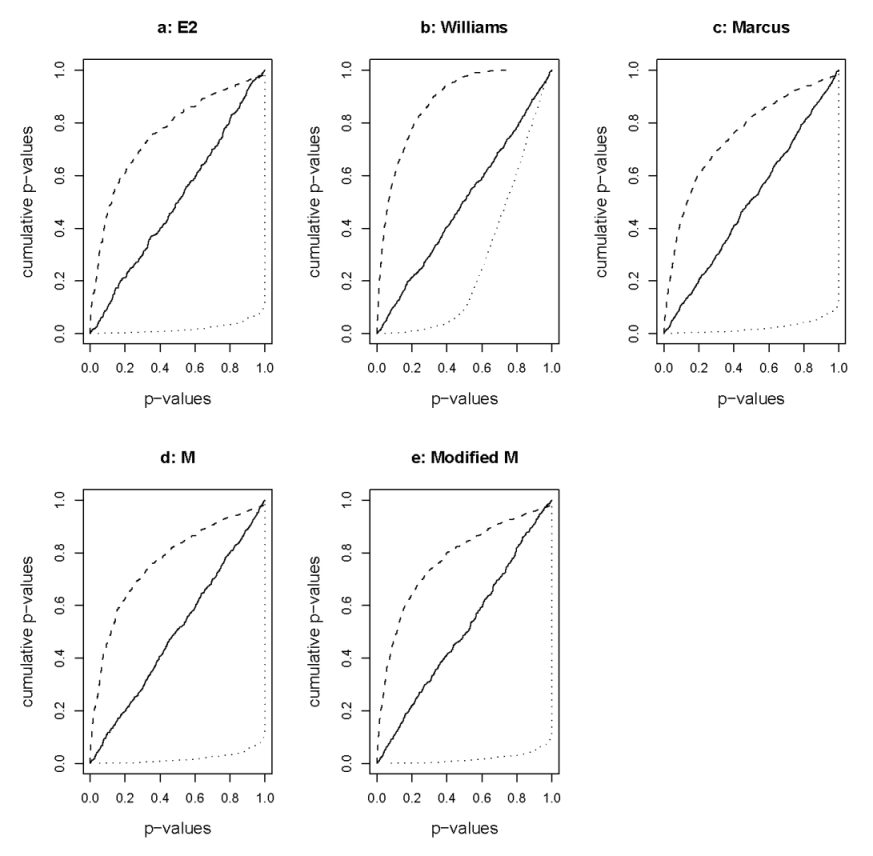
\includegraphics[width=1\textwidth]{pupdn1b.png}}
\caption{\em{The cumulative distribution of $p^{Up}$-values (dashed
line) and $p^{Down}$-values (dotted line) for the five test
statistics. Data are generated under $H_1^{Up}$ with isotonic means
(1, 2, 3, 4)/$\sqrt{5}$ for the four doses. Solid line: cumulative
distribution of $H_0\sim U[0,1]$.}} \label{pupdn1}
\end{figure}


Figure~\ref{stat1} shows the values of test statistics, which were
calculated under $H^{Up}_1$ and $H^{Down}_1$, for data generated
under $H^{Up}_1$. The five test statistics are calculated for
testing $H_0$ vs.\ $H^{Down}_1$ (the x-axis of each test statistic
in Figure~\ref{stat1}). The behavior of Marcus', $M$, and the
modified $M$ statistics is similar as they all use the difference
between the highest and the lowest isotonic mean.
%Marcus', $M$ and the modified $M$ test always forces the estimated trend to be decreasing or flat.
The maximum value of the test statistics (when calculated assuming
the wrong direction) is equal to zero. In contrast, Williams' test
statistic for testing $H_0$ vs.\ $H^{Down}_1$ (shown on the x-axis
of the panel $b$) can be positive or negative, because the sample
mean of control group is used instead of the isotonic mean. Note
that we reject the null hypothesis in favor of $H^{Down}_1$ for
negative values of the test statistic. Further, the value of the
test statistics for testing $H_0$ vs.\ $H^{Up}_1$ (the y-axis of
Figure~\ref{stat1}) is higher than the value of the test statistics
calculated for testing $H_0$ vs.\ $H^{Down}_1$ (the x-axis of
Figure~\ref{stat1}).



\begin{figure}[!h]
\centering
{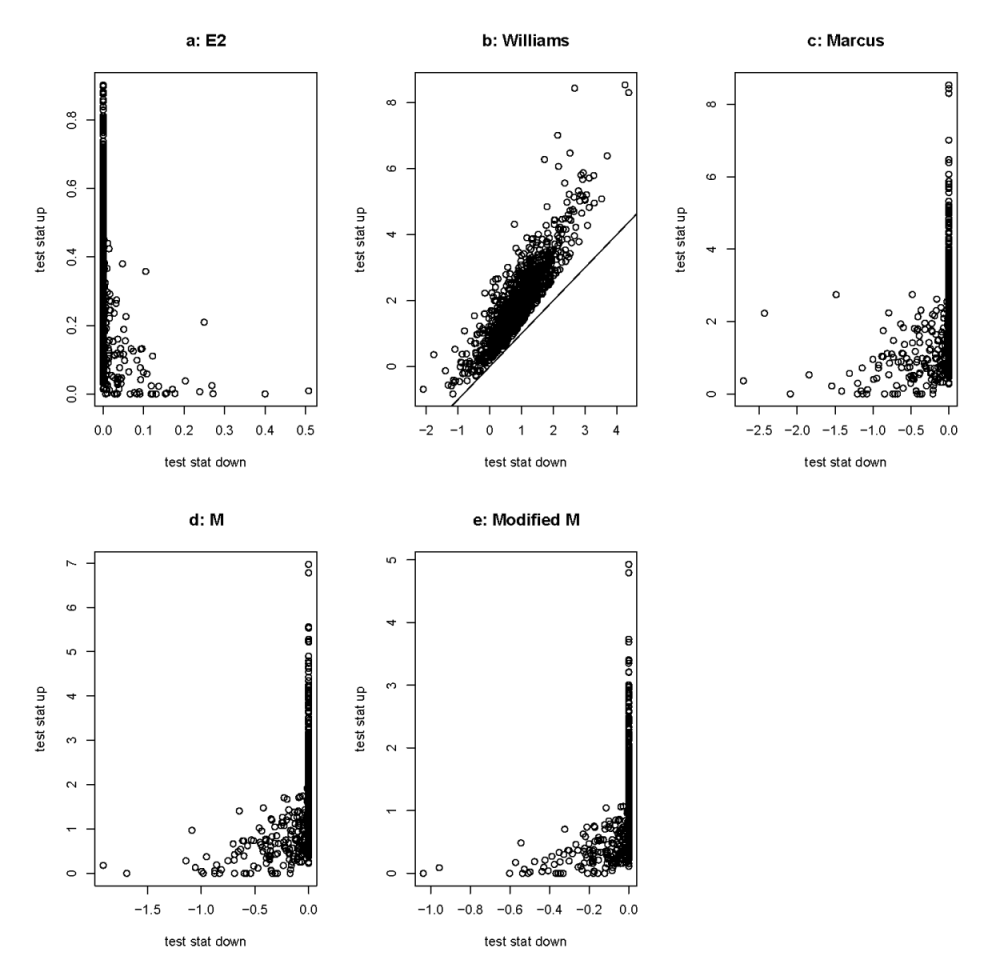
\includegraphics[width=1\textwidth]{stat1a.png}}
\caption{\em{The five test statistics calculated for $H_0$ vs.\
$H_1^{Up}$ (y-axis) and $H_0$ vs.\ $H_1^{Down}$ (x-axis).}}
\label{stat1}
\end{figure}








\subsection{Control of the Directional FDR}
\label{sec: FDR}

When the FDR controlling procedures are used to adjust for multiple
testing in the microarray setting, the set of two-sided $p$-values
computed for each gene is adjusted by using the BH-FDR or BY-FDR
procedure described in Section 3.2.1. A discovery in this case is a
rejection of $H_0$ for some gene; a false discovery is to reject
$H_0$ when $H_0$ is true. As mentioned before, in a microarray
dose-response experiment we are also interested in the direction of
the dose-response trend.

Benjamini and Yekutieli (2005)
% reference:
% \bibitem{BY} Benjamini Y., Yekutieli D., (2005a)
% ``False Discovery Rate-Adjusted Multiple Confidence Intervals for Selected Parameters''
% {\em Journal of the American Statistical Association}, {\bf 100}, 71-81.
provide a framework for addressing the multiplicity problem when
attempting to determine the direction of multiple parameters: a
discovery is to declare the sign of a parameter as either being
positive or negative. Three types of false discoveries are possible:
declaring a zero parameter either as negative or as positive,
declaring a negative parameter as positive, and declaring a positive
parameter as negative. The FDR corresponding to these discoveries is
termed the Mixed Directional FDR (MD-FDR). In the current setting,
the MD-FDR is the expected value of the number of genes, for which
$H_0$ is true, that are erroneously declared to have either a
positive or negative trend plus the genes with a monotone trend but
with a wrong direction of the declared trend, divided by the total
number of genes declared to have a trend. Benjamini and Yekutieli
(2005) prove that if $p$-values pose the directional property
described in Section~\ref{sec: directional}, then applying the BH
procedure at level $q$ to the the set of two-sided $p$-values
computed for each gene, and declaring the direction of the trend
corresponding to the smaller one-sided $p$-value, controls the
MD-FDR at level $q/2 \cdot (1 + m_0/m)$, where $m$ is the total
number of genes and $m_0$ is the number of genes, for which $H_0$
holds.

In general, directional inference is a more general setting than
hypotheses testing (Benjamini and Yekutieli, 2005). Nevertheless, as
a false discovery is made based on the $p$-value that is
stochastically larger than $U[0,1]$, then the resampling-based
methods that control the FDR (Yekutieli and Benjamini, 1999) also
control the MD-FDR. This is achieved by simply applying the
resampling-based procedure to test $H_0$, and if $H_0$ is rejected,
declaring the direction of the trend according to the minimum
one-sided $p$-value. For each rejected null hypothesis it is also
advisable to examine if the larger $p$-value is $\le \alpha$. If
this is the case, this may serve as an indication of a non-monotone
dose-response relationship.

%\chapter{The \texttt{IsoGene} Package in $R$}
%\markchapter{IsoGene R} \label{chap: isogene}

\section{Introduction to \texttt{IsoGene} Package}
\label{sec: intro}

%R is a language and a free software environment for statistical
%computing and graphics. It is a GNU project (a complete Unix-like
%operating system developed in 1984, which is free software) which is
%similar to the S language and environment which was developed at
%Bell Laboratories (formerly AT\&T, now Lucent Technologies) by John
%Chambers and colleagues. R can be considered as a different
%implementation of S. There are some important differences, but much
%code written for S runs unaltered under R.

%$R$ provides a wide variety of statistical and graphical techniques,
%and is highly extensible. It is an integrated suite of software
%facilities for data manipulation, calculation and graphical display.
%$R$, like $S$, is designed around a true computer language, and it
%allows users to add additional functionality by defining new
%functions. $R$ is an environment within which statistical techniques
%are implemented so that it can be extended (easily) via packages.
%The packages supplied with the $R$ distribution and many more are
%available through the Comprehensive R Archive Network (CRAN) family
%of Internet sites covering a very wide range of modern statistics.



%In this chapter, we present an $R$ package called \texttt{IsoGene}
%to implement the statistical methods discussed by Lin \textit{et
%al.}\ (2007), where the primary interest is testing for a monotonic
%relationship between gene-expressions and doses in a microarray
%experiment. %Lin \textit{et al.} discussed the five test statistics,
%including the global likelihood ratio test ($\bar{E}^2_{01}$,
%Bartholomew 1961, Barlow \textit{et al.} 1972, and Robertson
%\textit{et al.} 1988), Williams (1971, 1972), Marcus (1976), M (Hu
%\textit{et al.} 2005) and the modified M (Lin \textit{et al.} 2007)
%and using permutations to obtain the raw $p$-values of the test
%statistics and adjusting $p$-values using BH (Benjamini and Hochberg
%1995) and BY (Benjamini and Yekutilie 2001) procedures controlling
%FDR.


The main IsoGene package functions are \texttt{IsoRawp()} and
\texttt{IsoTestBH()}, which calculate the raw $p$-values using
permutations and adjust them using the BH- and BY-FDR procedures.
The supporting functions \texttt{IsoGene1()} and \texttt{IsoGenem()}
are used to calculate the five test statistics from isotonic
regression for one gene and all the genes, respectively. On the other hand,
the SAM procedure is also implemented to reduce some computational time as
compared to the permutation method. The main function of the SAM is \texttt{IsoTestSAM()},
with supporting functions \texttt{Isofudge(), IsoGenemSAM(), Isoqqstat(), Isoallfdr(), Isoqval()}.
The remaining functions \texttt{IsopvaluePlot(), IsoBHPlot(), IsoSAMPlot()
IsoPlot()} is used to display the data and
to show the results of testing procedures.

\section{Testing for Trends: Testing Procedures, Multiplicity and Resampling-based Inference}
\subsection{Resampling-based Multiple Testing}

\sloppy{For adjusting for multiple testing, only the BH-FDR procedure
(Benjamini and Hochberg 1995) and BY-FDR procedure (Benjamini and
Yekutieli 2001) are considered in package \texttt{IsoGene()}. The
matrix of the values of the test statistics for each gene and
permutation is referred as the permutation matrix under the null
distribution (see Section 3.2.2).}

% TODO: replace hard-coded sections

This matrix is used to calculate the one-sided $p$-values for the
inference. In the first step the one-sided raw (unadjusted for
multiple testing) $p^{Up}$-values are calculated using (\ref{p1}) or
(\ref{p2}) based on the test statistic $T^{Up}$.

\begin{equation}
P_i=\frac{\#(b: t_{ib} \ge t_{i})}{B-1}, \label{p1}
\end{equation}
where $t_i$ is the observed test statistic for gene $i$.

\begin{equation}
P_i=\frac{\sum_{b=1}^{B} \sum_{j=1}^{m} (t_{jb}\ge
t_{i})}{(B-1) \times m} \label{p2}.
\end{equation}

For $p^{Down}$-values, expect of $\bar{E}^2_{01}$, for which the
test statistic value $t_i$ is always between 0 and 1 and can be
obtained in the same way as $p^{Up}$-values,
\[p^{Down}=\#(b:t_{ib} \le t_{i})/B\; \mbox{or}\; p^{Down}=\sum_{b=1}^{B}
\sum_{j=1}^{m} (t_{jb} \le t_{i})/(B \times m)\] should be used
with $t_{ib}$ and $t_{jb}$ the test statistic values obtained for
gene $i$ and $j$ from permutation $b$. This is because under the
decreasing trend, we reject the four test statistics (namely,
Williams', Marcus', the $M$ and modified $M$) with large negative
values.

Based on the $p$-values, various methods adjusting the type I error
can be applied, such as the Bonferroni, Holm, Hochberg, and BH-FDR
and BY-FDR (Reiner \textit{et al.}\ 2003 and Ge \textit{et al.}\
2003).

\subsection{Significance Analysis of Microarray (SAM)}

SAM (Tusher \textit{et al.}\ 2001, Lin \textit{et al.}\ 2008) is a procedure widely used in the
microarray setting. SAM is a testing procedure, which estimates the
FDR by using permutations under the assumption that all null
hypotheses are true. The procedure consists of three components: (1)
the adjusted test statistics, (2) an approximation of the
distribution of the test statistics based on permutations, and (3)
the control of the FDR.

For a two-group setting, the modified test statistic in SAM is given
by,

\begin{equation}
t_{k}^{SAM}= \frac{\bar{x}_{k}-\bar{x}_{l}} {s_{k}+s_{0}},
\label{ttestSAM}
\end{equation}

where \[ \bar{x}_{l}=\frac{\Sigma_{j=1}^{n_{l}} x_{jl}}{n_{l}},\;\;
\bar{x}_{k}=\frac{\Sigma_{j=1}^{n_{k}} x_{jk}}{n_{k}},\;\;\]
\[s_{k}=\sqrt{\left (\frac{1}{n_{k}}+\frac{1}{n_{l}} \right )
{\frac{\Sigma_{j=1}^{n_{k}}
   (x_{jk}-\bar{x}_{jk})^2+\Sigma_{j=1}^{n_{l}}
   (x_{jl}-\bar{x}_{jl})^2}{n_{k}+n_{l}-2}}},
   \]
and $s_0$ is the fudge factor which is estimated from the data and
is discussed later, $k$ and $l$ are the index of the two groups of
array, and $j$ is the index of the array.

For $F$-type test statistic, such as $\bar{E}_{01}^2$, the modified test
statistic is given by,
\begin{equation}
\bar{E}_{01}^{2SAM}= \frac{\sqrt{\hat{\sigma}^2_{H_0}-\hat{\sigma}^2_{H_1}}} {\sqrt{\hat{\sigma}^2_{H_0}}+s_{0}},
\label{ttestSAM}
\end{equation}






SAM requires that the test statistic for each permutation is sorted
for all the genes, such that the first row of the sorted matrix is
the minimum test statistic across permutations, and the last row is
the maximum, i.e.,
\[\T^{SAM}= \left (
\begin{array}{llll}
t_{(1)1} & t_{(1)2} & \dots & t_{(1)B}\\
t_{(2)1} & t_{(2)2} & \dots & t_{(2)B}\\
.    & .    &.      & .     \\
.    & .    &.      & .     \\
.    & .    &.      & .     \\
t_{(m)1} & t_{(m)2} & \dots & t_{(m)B}\\
\end{array}
\right ).
\]

In $\T^{SAM}$, each element $t_{(i)b}$ is the sorted test statistic
for gene $i$ in permutation $b$. The expected values of the observed
ordered statistics are approximated by the means of the rows of
$\T^{SAM}$, given by $\bar{t}_{(1)}^{SAM}, \bar{t}_{(2)}^{SAM},
\dots, \bar{t}_{(m)}^{SAM}$ that are constructed in the following
way:
\[
\T^{SAM}= \left (
\begin{array}{llll}
t_{(1)1} & t_{(1)2} & \dots & t_{(1)B}\\ \hline t_{(2)1}
& t_{(2)2} & \dots & t_{(2)B}\\ \hline .    & . &.      & .
\\ \hline .    & .    &.      & .     \\ \hline . & .    &.      & .
\\ \hline
t_{(m)1} & t_{(m)2} & \dots & t_{(m)B}\\
\end{array}
\right ) \Rightarrow \left (
\begin{array}{l}
\frac{1}{B}\sum_{b=1}^{B}t_{(1)b} \\
\frac{1}{B}\sum_{b=1}^{B}t_{(2)b} \\
.                                     \\
.                                     \\
.                                     \\
\frac{1}{B}\sum_{b=1}^{B}t_{(m)b} \\
\end{array}
\right ) = \left (
\begin{array}{l}
\bar{t}_{(1)}^{SAM} \\
\bar{t}_{(2)}^{SAM} \\
.                                     \\
.                                     \\
.                                     \\
\bar{t}_{(m)}^{SAM} \\
\end{array}
\right ).
\]

%\noindent \textbf{SAM Procedure}

The SAM procedure proposed by Tusher \textit{et al.}\ (2001) is as
follows:

\begin{enumerate}

\item Compute order statistics $t_{(1)}^{SAM} \le t_{(2)}^{SAM} \le
\dots \le t_{(m)}^{SAM}$.

\item Compute the permutation matrix $\T^{SAM}$.

\item Calculate the expected test statistics
$\bar{t}_{(1)}^{SAM},\bar{t}_{(2)}^{SAM},\dots,\bar{t}_{(m)}^{SAM}$.

\item Plot the $t_{(1)}^{SAM} , t_{(2)}^{SAM}, \dots , t_{(m)}^{SAM}$
values versus the
$\bar{t}_{(1)}^{SAM},\bar{t}_{(2)}^{SAM},\dots,\bar{t}_{(m)}^{SAM}$
values (SAM plot).

\item For a fixed threshold $\Delta$, starting at the origin, and
moving up to the right, find the first $i=i_1$ such that
$t_i^{SAM}-\bar{t}_{i}^{SAM} > \Delta$. All genes, for which
$t_i^{SAM}$ $>$ $t_{i1}^{SAM}$, are called ``significant positive".
Similarly, start at origin, move down to the left and find the first
$i=i_2$ such that $\bar{t}_{2}^{SAM}-t_i^{SAM}> \Delta$. All genes,
for which $t_i^{SAM}$ $<$ $t_{i2}^{SAM}$, are called ``significant
negative". For each $\Delta$ define the upper cut-point
C$_{up}(\Delta)$ as the smallest $t_i^{SAM}$ among the significant
positive genes, and similarly define the lower cut-point
C$_{low}(\Delta)$.

\item For a grid of $\Delta$ values, compute the total number of
significant genes (from step 5), and the median number of falsely
called genes, i.e., the median number of values among each of the
$B$ sets of $t_{ib}$ , $i=1,2,\dots,m$ that fall above cut-point
C$_{up}(\Delta)$ and below cut-point C$_{down}(\Delta)$.
Similarly, compute the $90$th percentile of the number of falsely
called genes.

\item Estimate $\pi_0$, the proportion of truly non-differentially
expressed genes in the data set, as follows:

\begin{enumerate}

\item Compute the first and third quantiles of the permuted
$t^{SAM}$ values, denoted as $q25$ and $q75$ (the $t_i^{SAM}$ are
the values for the original data set; there are $m$ such values).

\item Compute  $\hat{\pi}_0 = \# \{ t_{i} \in (q25, q75)\} / (.5m)$.

\item Let $\hat{\pi}_0 = min (\hat{\pi}_0 , 1)$.
\end{enumerate}

\item  The median and the $90$th percentile of the number of falsely
called genes from step 6, are multiplied by $\hat{\pi}_0$,

\item Pick a $\Delta$ and the corresponding number of significant genes.


\item The FDR is estimated by the median (or the $90$th percentile) of the
number of falsely called genes divided by the number of significant
genes.


%\item $q$-value is the lowest FDR, at which a gene is called
%``significant". It resembles the $p$-value, but is adapted to the
%analysis of a large number of genes. Note that as $ t^{SAM}_i> 0$
%increases, the corresponding $q$-value decreases.

\end{enumerate}


\noindent \textbf{Estimation of the SAM Fudge Factor $s_0$}

In the procedure described above, a fudge factor $s_0$ in the
denominator of the test statistic~(\ref{ttestSAM}) is used. It is
calculated as the percentile of the gene-wise standard error
distribution that minimizes the coefficient of variation (CV) of the
test statistics. This modification is used to overcome bias for
genes with expressions close to zero, which have a large value of
the test statistic due to a small sample variance. By using an
inflated standard error, SAM addresses the problem of the dependence
of the value of the test statistic on the variance of expression
levels for a particular gene. The calculation of $s_0$ is as
follows:

\begin{enumerate}

\item Let $s_{\alpha}$ be the $\alpha \cdot 100\%$ percentile of $s_i$ values.
Let $t_i^{\alpha}= (\bar{X}_{1}-\bar{X}_{0})/(s_i+s_{\alpha})$.

\item Compute the 100 centiles of the $s_i$ values, denoted by $q_1 <
q_2\dots < q_{100}$.

\item For $\alpha \in (0, 0.05, 0.10, \dots, 1.0)$

\begin{enumerate}

\item compute $\nu_j= \mbox{MAD}(t_i^{\alpha}|s_i \in
[q_j,q_{j+1})),j=1,2,\dots,m$, where \mbox{MAD} is the median
absolute deviation from the median, divided by .64;

\item compute $cv(\alpha)=$ coefficient of variation of the $\nu_j$
values.

\end{enumerate}

\item Choose $\hat{\alpha}=argmin[cv(\alpha)]$, i.e.,
$\hat{\alpha}$ is the quantile of the standard error that minimizes
the coefficient of variation of the SAM test statistics.

\item Compute $\hat{s}_0=s_{\hat{\alpha}}$.

\end{enumerate}




\section{Using the \texttt{IsoGene} Package}

\subsection{Data Example}

The data used for the analysis presented below are outcome of a dose-response microarray experiment
consisting of four dose levels. Three microarray samples are available at each dose level (hence, in total
gene expression was measured for 12 arrays). Each array consists of 16,998 genes.

A dataframe with the log2 transformed gene intensities is loaded
into $R$ environment. The first ten genes and first six samples are
displayed, where the row names of the genes show the probe ID,
\texttt{X1, X1.1 and X1.2} are the three arrays for dose zero, while
\texttt{X2, X2.1 and X2.2} are the arrays for the first dose. The dataframe is loaded suing the function \texttt{load()},
\begin{center}
\begin{boxit}
\begin{verbatim}
> load("data.Rdata")
\end{verbatim}
\end{boxit}
\end{center}
A printout of the first 10 lines is given below.
\begin{center}
\begin{boxit}
\begin{verbatim}
> data[1:10,1:6]
                 X1     X1.1     X1.2       X2     X2.1     X2.2
g1 6.923109 7.024719 7.170328 7.219297 7.076908 7.404949
g2 5.107275 5.092935 5.255918 5.312913 4.893855 4.596591
g3 5.913526 6.026197 5.141728 5.828770 5.269202 5.461664
g4   4.919469 4.908159 3.500307 4.814068 4.139949 4.278321
g5   6.002091 5.878718 5.777668 6.214799 5.895586 6.163291
g6 7.162715 7.294693 6.903935 7.223069 6.972928 7.412160
g7   4.049696 4.748409 3.845498 4.780287 4.076589 4.300242
g8   3.191931 4.326571 3.771206 3.570291 2.179324 3.988911
g9   6.487708 6.285804 6.229814 6.109103 6.340837 5.931840
g10   6.695870 6.687039 6.652153 6.503670 6.387794 6.698711
\end{verbatim}
\end{boxit}
\end{center}

\subsection{Loading the Package}

\sloppypar {To load the \texttt{IsoGene} package into $R$, a binary
zip-package of \texttt{IsoGene} program (for Windows) needs to be
installed. \texttt{IsoGene} package requires $R$ packages
\texttt{Multtest} and \texttt{ff}, which need to be installed as
well. Once the packages are installed, they are available for use
after being loaded in memory, which is usually done by the user:}

\begin{Schunk}
\begin{Sinput}
> library(IsoGene)
\end{Sinput}
\begin{Soutput}
Loading package ff
- getOption("fftempdir")=="C:/Users/lucp1618/AppData/Local/Temp/RtmpzYHFpW"
- getOption("fffinonexit")==TRUE
- getOption("ffpagesize")==65536
- getOption("ffcaching")=="mmnoflush"
- getOption("ffdrop")==TRUE
- getOption("ffbatchbytes")==16104816
Attaching package ff
\end{Soutput}
\end{Schunk}

The functions included in the package can be listed using the $R$
help system:

\begin{Schunk}
\begin{Sinput}
> help(package = IsoGene)
\end{Sinput}
\end{Schunk}

%\begin{figure}[!h]
%\centering
%{\subfigure{\resizebox{.89\textwidth}{!}{\includegraphics{D:/Data/Ph.Dthesis/Figures/IsoGeneLib/page1.eps}}}\\
%\subfigure{\resizebox{.9\textwidth}{!}{\includegraphics{D:/Data/Ph.Dthesis/Figures/IsoGeneLib/page2.eps}}}
%} \caption{\em{The main help file of IsoGene package.}}
%\label{IsoGeneHelp}
%\end{figure}



%\begin{figure}[!h]
%\centering
%{\includegraphics[width=.6\textwidth]{IsoGenehelp.eps}}
%\caption{\em{The main help file of IsoGene package.}}
%\label{IsoGeneHelp}
%\end{figure}


%The help file of \texttt{IsoGene} package is shown in
%Figure~\ref{IsoGeneHelp}.
First, \texttt{IsoPlot()} can be used to
explore the data. Second, \texttt{IsoGene1()} and
\texttt{IsoGenem()} can be used to calculate the test statistics.
Third, \texttt{IsoRawp()} provides the output for two-sided or
one-sided $p$-values ($p^{Up}$ or $p^{Down}$). Based on the
$p$-values obtained, one can choose one test statistic and
multiplicity adjustment method for inference by using
\texttt{IsoTestBH()}. Finally, \texttt{IsopvaluePlot()} can be
useful for examining both of $p^{Up}$- or $p^{Down}$-values, and in
particularly, as a post hoc procedure it can be used to examine
genes with both small $p^{Up}$- and $p^{Down}$-values.


\section{The \texttt{IsoGene} Functions}
\subsection{Quick Start}
The first stage of the analysis (which is also the time consuming stage) consists of permutations under the null hypothesis in order to obtain the distribution of the test statistic under the null hypothesis. Note that, by default, all five test statistics discussed above are calculated. The function \texttt{IsoRawp()} is used to perform the permutation. A general call of the function \texttt{IsoRawp()} has the form of
\begin{center}
\begin{boxit}
\begin{verbatim}
IsoRawp(x, data, niter=1000)
\end{verbatim}
\end{boxit}
\end{center}
Here, \texttt{x} is a vector which contains the dose levels and \texttt{data} is the R object, which contains the information about gene expression and genes names. Once the permutation stage is completed, the FDR adjusted $p$-values can be obtained using function \texttt{IsoTestBH()}. The function calculates the adjusted p values for each statistic using either the BH-FDR or BY-FDR for multiplicity adjustment. The user can specify one of the five test statistics discussed above, or use the default call, in the later case adjusted $p$-values for all test statistics will be calculated. A general form of the \texttt{IsoTestBH()} has the form
\begin{center}
\begin{boxit}
\begin{verbatim}
IsoTestBH(rp, FDR=c(0.05,0.1), type=c("BH","BY"),
stat=c("E2","Williams","Marcus","M","ModifM"))
\end{verbatim}
\end{boxit}
\end{center}
Note that \texttt{rp} is an R object, which contains all the output produced by the function \texttt{IsoRawp()}.\newline In what follows we illustrate in more details the use of the functions of the \texttt{IsoGene} package.

\subsection{Exploring the Data}

\texttt{IsoPlot()} can be used to explore the data. Scatterplots for the
second gene in the dataset (\texttt{data[2,]}) can be produced by

\begin{Schunk}
\begin{Sinput}
> data(exampleData)
\end{Sinput}
\end{Schunk}


\begin{Schunk}
\begin{Sinput}
> x <- c(rep(1, 3), rep(2, 3), rep(3, 3), rep(4, 3))
> gene1 <- as.matrix(exampleData[2, ])
> par(mfrow = c(1, 2))
> IsoPlot(x, y = gene1)
> IsoPlot(x, y = gene1, type = "ordinal", add.curve = TRUE)
\end{Sinput}
\end{Schunk}
 
 
 

\begin{figure}[!h]
\centering
{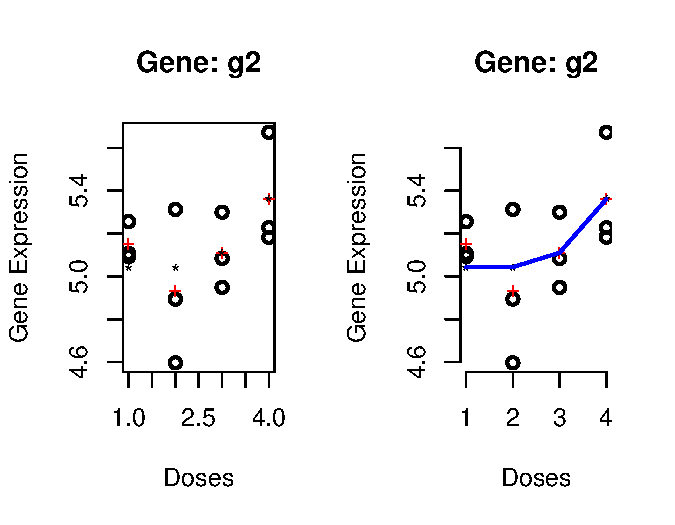
\includegraphics[width=0.8\textwidth]{IsoGene-IsoPlot.pdf}}
\caption{\em{The data points are plotted as circles, while sample
means as pluses. The right panel additionally plots the fitted
increasing isotonic regression model (blue solid line).}}
\label{exgene}
\end{figure}




The left panel in Figure~\ref{exgene} shows the original data points
(as circles) and sample means (as pluses) for each dose. The right
panel in Figure~\ref{exgene} shows the increasing isotonic
regression model (blue solid line) fitted on the data. The fitted
monotonic line does not indicate the significance of the test, but
simply shows a more likely increasing (or decreasing) trend.


\subsection{Calculating the Test Statistics}

The five test statistics described in Chapter 2 can be obtained by
using the function \texttt{IsoGene1()} for a single gene and using
the function \texttt{IsoGenem()} for all the genes simultaneously.
The following $R$ codes illustrate the input and output generated by
these two functions:

\begin{Schunk}
\begin{Sinput}
> stat1 <- IsoGene1(x, gene1)
\end{Sinput}
\end{Schunk}

The object \texttt{stat1} contains the information about the five test statistics and the direction for which the likelihood is maximizes.

\begin{Schunk}
\begin{Sinput}
> stat1
\end{Sinput}
\begin{Soutput}
$E2.up
[1] 0.2697894

$Williams.up
[1] 1.040134

$Marcus.up
[1] 1.581191

$M.up
[1] 1.205802

$ModM.up
[1] 1.278946

$E2.dn
[1] 0.0008106545

$Williams.dn
[1] -0.08238646

$Marcus.dn
[1] -0.08238646

$M.dn
[1] -0.05370908

$ModM.dn
[1] -0.06004858

$direction
[1] "u"
\end{Soutput}
\end{Schunk}

The first 10 objects are the values calculated for the five test
statistics under increasing and decreasing trends. The last object
indicates the higher likelihood of isotonic regression with ``u"
meaning a increasing trend or ``d" meaning a decreasing trend.


We use the first 10 genes as an example to illustrate the use of
function \texttt{IsoGenem()}:

\begin{Schunk}
\begin{Sinput}
> statm <- IsoGenem(x, exampleData[1:10, ])
> statm
\end{Sinput}
\begin{Soutput}
$E2.up
        g1         g2         g3         g4         g5         g6         g7 
0.81527841 0.26978939 0.81226244 0.04625381 0.02356596 0.01270386 0.00000000 
        g8         g9        g10 
0.05438655 0.02259598 0.99060602 

$Williams.up
 [1]  5.706246398  1.040133583  4.532537020  0.485215821  0.546648138
 [6]  0.357615051 -0.134476246 -0.009111866 -0.693505488 28.489753149

$Marcus.up
 [1]  5.7062464  1.5811905  5.0052320  0.5279040  0.5466481  0.3576151
 [7]  0.0000000  0.5170096  0.4308062 29.4025214

$M.up
 [1]  4.6591307  1.2058018  3.9221693  0.4308356  0.2929374  0.2138936
 [7]  0.0000000  0.3916276  0.2867030 20.1706306

$ModM.up
 [1]  4.6591307  1.2789459  4.3851186  0.4569702  0.3275140  0.2391403
 [7]  0.0000000  0.4378530  0.3205437 21.3941846

$E2.dn
          g1           g2           g3           g4           g5           g6 
0.0000000000 0.0008106545 0.0000000000 0.0000000000 0.3328630108 0.3126307156 
          g7           g8           g9          g10 
0.0902853975 0.0194293995 0.2236936672 0.0000000000 

$Williams.dn
 [1]  2.47954450 -0.08238646  0.77861303  0.15969984 -1.08594004 -1.06231999
 [7] -0.45383921 -0.35682222 -1.35548019  7.55960274

$Marcus.dn
 [1]  0.00000000 -0.08238646  0.00000000  0.00000000 -2.16867670 -1.77404170
 [7] -0.63872592 -0.35682222 -1.35548019  0.00000000

$M.dn
 [1]  0.00000000 -0.05370908  0.00000000  0.00000000 -1.40596911 -1.27167021
 [7] -0.51444688 -0.26542632 -1.01219460  0.00000000

$ModM.dn
 [1]  0.00000000 -0.06004858  0.00000000  0.00000000 -1.49125543 -1.42177051
 [7] -0.57516910 -0.29675565 -1.13166796  0.00000000

$direction
 g1  g2  g3  g4  g5  g6  g7  g8  g9 g10 
"u" "u" "u" "u" "d" "d" "d" "u" "d" "u" 
\end{Soutput}
\end{Schunk}


The output from \texttt{IsoGenem()} has the same structure as the one
for \texttt{IsoGene1()}, but each object contains the values of the
test statistics and the likely direction of the isotonic regression
model for all the genes.


\subsection{Obtaining Raw $p$-values}

As discussed above, we use permutations to obtain the raw $p$-values
for the five test statistics. The function \texttt{IsoRawp()} can be
used in the following way:

\begin{Schunk}
\begin{Sinput}
> rawp <- IsoRawp(x = x, y = exampleData, niter = 2)
\end{Sinput}
\end{Schunk}


The four arguments in this function need to be specified, with no
default pre-specified values. \texttt{x} is the explanatory variable
indicating the dose levels for all the samples in the data.
\texttt{data} is the data frame of gene expression values. % TODO remove "data frame"
\texttt{niter} defines the number of permutations used to
approximate the null distribution. The output item
\texttt{rawp} contains four objects with $p$-values for the five
test statistics: the first one contains the two-sided $p$-values,
the second contains the one-sided $p$-values, the third contains
$p^{Up}$-values, and the last one contains $p^{Down}$-values. Below
we print a part of the object with two-sided $p$-values for illustration:

\begin{Schunk}
\begin{Sinput}
> rawp.twosided <- rawp[[1]]
\end{Sinput}
\end{Schunk}


The first 10 rows in of the object \texttt{rawp.twosided} are
\begin{Schunk}
\begin{Sinput}
> rawp.twosided[1:10, ]
\end{Sinput}
\begin{Soutput}
   Probe.ID  E2 Williams Marcus   M ModM
1        g1 0.0      0.0    0.0 0.0  0.0
2        g2 0.0      0.0    0.0 0.0  0.0
3        g3 0.0      0.0    0.0 0.0  0.0
4        g4 0.5      0.5    0.5 0.5  0.5
5        g5 0.0      0.0    0.0 0.0  0.0
6        g6 0.0      0.0    0.0 0.0  0.0
7        g7 0.0      0.0    0.0 0.0  0.0
8        g8 0.0      0.5    0.5 0.5  0.0
9        g9 0.5      0.5    0.5 0.5  0.5
10      g10 0.0      0.0    0.0 0.0  0.0
\end{Soutput}
\end{Schunk}


The first output object from \texttt{rawp} is a matrix with six
columns, where the first column indicates the probe ID. Columns from
the second to the sixth are $p$-values for each of the five test
statistics, respectively. The remaining three output objects
(\texttt{rawp}[[2]], \texttt{rawp}[[3]], \texttt{rawp}[[4]]) are
structured in the same way.


\subsection{Plot of $p$-values for a Single Gene}

For a single gene, the function \texttt{IsopvaluePlot()} can be used
to show the $p^{Up}$ and $p^{Down}$-values for a given test
statistic:

\begin{Schunk}
\begin{Sinput}
> IsopvaluePlot(x, y, niter, stat = c("E2", "Williams", "Marcus", 
+     "M", "ModifM"))
\end{Sinput}
\end{Schunk}


We use one gene as an example to illustrate how $p^{Up}$ and
$p^{Down}$-values (in the upper and lower panels of
Figure~\ref{expvalue}) are obtained. In Figure~\ref{expvalue}, the
observed test statistics are drawn as the dashed line, and the
values of the test statistics obtained from permutations are spread
over the x-axis. For this gene, the $p^{Up}$ is much smaller as
compared to the $p^{Down}$ since $T^{Up} \gg T^{Down}$, which
implies a possible increasing trend in the data.

\begin{Schunk}
\begin{Sinput}
> IsopvaluePlot(x, gene1, niter = 1000, stat = "E2")
\end{Sinput}
\end{Schunk}


\begin{Schunk}
\begin{Soutput}
1 . 2 . 3 . 4 . 5 . 6 . 7 . 8 . 9 . 10 . 11 . 12 . 13 . 14 . 15 . 16 . 17 . 18 . 19 . 20 . 21 . 22 . 23 . 24 . 25 . 26 . 27 . 28 . 29 . 30 . 31 . 32 . 33 . 34 . 35 . 36 . 37 . 38 . 39 . 40 . 41 . 42 . 43 . 44 . 45 . 46 . 47 . 48 . 49 . 50 . 51 . 52 . 53 . 54 . 55 . 56 . 57 . 58 . 59 . 60 . 61 . 62 . 63 . 64 . 65 . 66 . 67 . 68 . 69 . 70 . 71 . 72 . 73 . 74 . 75 . 76 . 77 . 78 . 79 . 80 . 81 . 82 . 83 . 84 . 85 . 86 . 87 . 88 . 89 . 90 . 91 . 92 . 93 . 94 . 95 . 96 . 97 . 98 . 99 . 100 . 101 . 102 . 103 . 104 . 105 . 106 . 107 . 108 . 109 . 110 . 111 . 112 . 113 . 114 . 115 . 116 . 117 . 118 . 119 . 120 . 121 . 122 . 123 . 124 . 125 . 126 . 127 . 128 . 129 . 130 . 131 . 132 . 133 . 134 . 135 . 136 . 137 . 138 . 139 . 140 . 141 . 142 . 143 . 144 . 145 . 146 . 147 . 148 . 149 . 150 . 151 . 152 . 153 . 154 . 155 . 156 . 157 . 158 . 159 . 160 . 161 . 162 . 163 . 164 . 165 . 166 . 167 . 168 . 169 . 170 . 171 . 172 . 173 . 174 . 175 . 176 . 177 . 178 . 179 . 180 . 181 . 182 . 183 . 184 . 185 . 186 . 187 . 188 . 189 . 190 . 191 . 192 . 193 . 194 . 195 . 196 . 197 . 198 . 199 . 200 . 201 . 202 . 203 . 204 . 205 . 206 . 207 . 208 . 209 . 210 . 211 . 212 . 213 . 214 . 215 . 216 . 217 . 218 . 219 . 220 . 221 . 222 . 223 . 224 . 225 . 226 . 227 . 228 . 229 . 230 . 231 . 232 . 233 . 234 . 235 . 236 . 237 . 238 . 239 . 240 . 241 . 242 . 243 . 244 . 245 . 246 . 247 . 248 . 249 . 250 . 251 . 252 . 253 . 254 . 255 . 256 . 257 . 258 . 259 . 260 . 261 . 262 . 263 . 264 . 265 . 266 . 267 . 268 . 269 . 270 . 271 . 272 . 273 . 274 . 275 . 276 . 277 . 278 . 279 . 280 . 281 . 282 . 283 . 284 . 285 . 286 . 287 . 288 . 289 . 290 . 291 . 292 . 293 . 294 . 295 . 296 . 297 . 298 . 299 . 300 . 301 . 302 . 303 . 304 . 305 . 306 . 307 . 308 . 309 . 310 . 311 . 312 . 313 . 314 . 315 . 316 . 317 . 318 . 319 . 320 . 321 . 322 . 323 . 324 . 325 . 326 . 327 . 328 . 329 . 330 . 331 . 332 . 333 . 334 . 335 . 336 . 337 . 338 . 339 . 340 . 341 . 342 . 343 . 344 . 345 . 346 . 347 . 348 . 349 . 350 . 351 . 352 . 353 . 354 . 355 . 356 . 357 . 358 . 359 . 360 . 361 . 362 . 363 . 364 . 365 . 366 . 367 . 368 . 369 . 370 . 371 . 372 . 373 . 374 . 375 . 376 . 377 . 378 . 379 . 380 . 381 . 382 . 383 . 384 . 385 . 386 . 387 . 388 . 389 . 390 . 391 . 392 . 393 . 394 . 395 . 396 . 397 . 398 . 399 . 400 . 401 . 402 . 403 . 404 . 405 . 406 . 407 . 408 . 409 . 410 . 411 . 412 . 413 . 414 . 415 . 416 . 417 . 418 . 419 . 420 . 421 . 422 . 423 . 424 . 425 . 426 . 427 . 428 . 429 . 430 . 431 . 432 . 433 . 434 . 435 . 436 . 437 . 438 . 439 . 440 . 441 . 442 . 443 . 444 . 445 . 446 . 447 . 448 . 449 . 450 . 451 . 452 . 453 . 454 . 455 . 456 . 457 . 458 . 459 . 460 . 461 . 462 . 463 . 464 . 465 . 466 . 467 . 468 . 469 . 470 . 471 . 472 . 473 . 474 . 475 . 476 . 477 . 478 . 479 . 480 . 481 . 482 . 483 . 484 . 485 . 486 . 487 . 488 . 489 . 490 . 491 . 492 . 493 . 494 . 495 . 496 . 497 . 498 . 499 . 500 . 501 . 502 . 503 . 504 . 505 . 506 . 507 . 508 . 509 . 510 . 511 . 512 . 513 . 514 . 515 . 516 . 517 . 518 . 519 . 520 . 521 . 522 . 523 . 524 . 525 . 526 . 527 . 528 . 529 . 530 . 531 . 532 . 533 . 534 . 535 . 536 . 537 . 538 . 539 . 540 . 541 . 542 . 543 . 544 . 545 . 546 . 547 . 548 . 549 . 550 . 551 . 552 . 553 . 554 . 555 . 556 . 557 . 558 . 559 . 560 . 561 . 562 . 563 . 564 . 565 . 566 . 567 . 568 . 569 . 570 . 571 . 572 . 573 . 574 . 575 . 576 . 577 . 578 . 579 . 580 . 581 . 582 . 583 . 584 . 585 . 586 . 587 . 588 . 589 . 590 . 591 . 592 . 593 . 594 . 595 . 596 . 597 . 598 . 599 . 600 . 601 . 602 . 603 . 604 . 605 . 606 . 607 . 608 . 609 . 610 . 611 . 612 . 613 . 614 . 615 . 616 . 617 . 618 . 619 . 620 . 621 . 622 . 623 . 624 . 625 . 626 . 627 . 628 . 629 . 630 . 631 . 632 . 633 . 634 . 635 . 636 . 637 . 638 . 639 . 640 . 641 . 642 . 643 . 644 . 645 . 646 . 647 . 648 . 649 . 650 . 651 . 652 . 653 . 654 . 655 . 656 . 657 . 658 . 659 . 660 . 661 . 662 . 663 . 664 . 665 . 666 . 667 . 668 . 669 . 670 . 671 . 672 . 673 . 674 . 675 . 676 . 677 . 678 . 679 . 680 . 681 . 682 . 683 . 684 . 685 . 686 . 687 . 688 . 689 . 690 . 691 . 692 . 693 . 694 . 695 . 696 . 697 . 698 . 699 . 700 . 701 . 702 . 703 . 704 . 705 . 706 . 707 . 708 . 709 . 710 . 711 . 712 . 713 . 714 . 715 . 716 . 717 . 718 . 719 . 720 . 721 . 722 . 723 . 724 . 725 . 726 . 727 . 728 . 729 . 730 . 731 . 732 . 733 . 734 . 735 . 736 . 737 . 738 . 739 . 740 . 741 . 742 . 743 . 744 . 745 . 746 . 747 . 748 . 749 . 750 . 751 . 752 . 753 . 754 . 755 . 756 . 757 . 758 . 759 . 760 . 761 . 762 . 763 . 764 . 765 . 766 . 767 . 768 . 769 . 770 . 771 . 772 . 773 . 774 . 775 . 776 . 777 . 778 . 779 . 780 . 781 . 782 . 783 . 784 . 785 . 786 . 787 . 788 . 789 . 790 . 791 . 792 . 793 . 794 . 795 . 796 . 797 . 798 . 799 . 800 . 801 . 802 . 803 . 804 . 805 . 806 . 807 . 808 . 809 . 810 . 811 . 812 . 813 . 814 . 815 . 816 . 817 . 818 . 819 . 820 . 821 . 822 . 823 . 824 . 825 . 826 . 827 . 828 . 829 . 830 . 831 . 832 . 833 . 834 . 835 . 836 . 837 . 838 . 839 . 840 . 841 . 842 . 843 . 844 . 845 . 846 . 847 . 848 . 849 . 850 . 851 . 852 . 853 . 854 . 855 . 856 . 857 . 858 . 859 . 860 . 861 . 862 . 863 . 864 . 865 . 866 . 867 . 868 . 869 . 870 . 871 . 872 . 873 . 874 . 875 . 876 . 877 . 878 . 879 . 880 . 881 . 882 . 883 . 884 . 885 . 886 . 887 . 888 . 889 . 890 . 891 . 892 . 893 . 894 . 895 . 896 . 897 . 898 . 899 . 900 . 901 . 902 . 903 . 904 . 905 . 906 . 907 . 908 . 909 . 910 . 911 . 912 . 913 . 914 . 915 . 916 . 917 . 918 . 919 . 920 . 921 . 922 . 923 . 924 . 925 . 926 . 927 . 928 . 929 . 930 . 931 . 932 . 933 . 934 . 935 . 936 . 937 . 938 . 939 . 940 . 941 . 942 . 943 . 944 . 945 . 946 . 947 . 948 . 949 . 950 . 951 . 952 . 953 . 954 . 955 . 956 . 957 . 958 . 959 . 960 . 961 . 962 . 963 . 964 . 965 . 966 . 967 . 968 . 969 . 970 . 971 . 972 . 973 . 974 . 975 . 976 . 977 . 978 . 979 . 980 . 981 . 982 . 983 . 984 . 985 . 986 . 987 . 988 . 989 . 990 . 991 . 992 . 993 . 994 . 995 . 996 . 997 . 998 . 999 . 1000 . 
\end{Soutput}
\end{Schunk}
 
  
\begin{figure}[!h]
\centering
{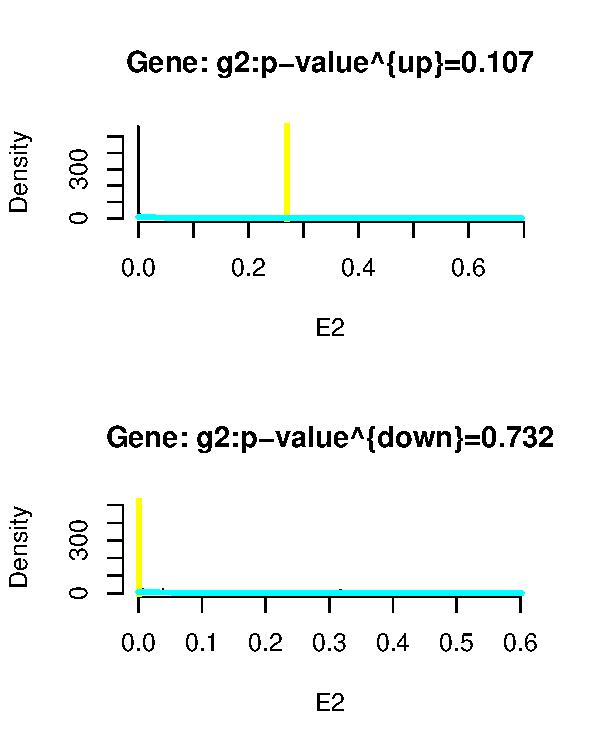
\includegraphics[width=0.8\textwidth]{IsoGene-IsopvaluePlot.pdf}}
\caption{\em{The $p^{Up}$ and $p^{Down}$-values using
$\bar{E}_{01}^2$ for an example gene. The dashed line is the
observed test statistic value. In the upper panel, the dashed line
(at the right) is larger than most of the test statistics from
permutations, which results in a small $p^{Up}$-value. In the lower
panel, the dashed line (close to zero) is smaller than most of the
test statistics from permutations, which results in a large
$p^{Down}$-value.}} \label{expvalue}
\end{figure}



\subsection{BH/BY-FDR Procedures for Adjusting for Multiple Testing}

With the two-sided $p$-values, the user needs to select one of the
five test statistics, the FDR level, and the type of multiplicity
adjustment (BH-FDR or BY-FDR) to obtain the list of significant
genes:

\begin{Schunk}
\begin{Sinput}
> IsoTestBH(rp, FDR = c(0.05, 0.1), type = c("BH", "BY"), stat = c("E2", 
+     "Williams", "Marcus", "M", "ModifM"))
\end{Sinput}
\end{Schunk}


The following example shows the use of the global likelihood ratio
test $\bar{E}^{2}_{01}$, the FDR level of 0.05 and the BH-FDR
procedure controlling the FDR: \\ \\

\begin{Schunk}
\begin{Sinput}
> E2.BH <- IsoTestBH(rawp.twosided, FDR = 0.05, type = "BH", stat = "E2")
\end{Sinput}
\end{Schunk}

The first 10 rows in the object \texttt{E2.BH} list the sorted row and adjusted p values for the $\bar{E}^{2}_{01}$ statistic.

\begin{Schunk}
\begin{Sinput}
> E2.BH[1:10, ]
\end{Sinput}
\begin{Soutput}
   Probe.ID row.name raw p-values BH adjusted p values
1        g1        1            0                    0
2        g2        2            0                    0
3        g3        3            0                    0
4        g5        5            0                    0
5        g6        6            0                    0
6        g7        7            0                    0
7        g8        8            0                    0
8       g10       10            0                    0
9       g11       11            0                    0
10      g12       12            0                    0
\end{Soutput}
\end{Schunk}
%s

Here we show only the first ten genes declared significant by using
$\bar{E}^{2}_{01}$ test. The output results in a matrix of five
columns: the first column indicates the probe ID, the second column
is the corresponding row number of significant genes in the original
dataset, the third column is the unadjusted/raw $p$-value, and the
last column is the adjusted $p$-value using the requested ``BH"
procedure. The order of the list of genes found significant is based
on the row number. Moreover, the function \texttt{IsoBHPlot()} can
be used to visualize the number of significant findings for the
BH-FDR and BY-FDR procedures for the specified test statistic:

\begin{Schunk}
\begin{Sinput}
> IsoBHPlot(rp, FDR = c(0.05, 0.1), stat = c("E2", "Williams", 
+     "Marcus", "M", "ModifM"))
\end{Sinput}
\end{Schunk}

Figure~\ref{IsoBHPlot} shows the unadjusted (solid blue line) and
the BH-FDR (dotted and dashed red line) and BY-FDR (dashed green
line) adjusted $p$-values for $\bar{E}^2_{01}$. It is obtained using
the function \texttt{IsoBHPlot()}:

\begin{Schunk}
\begin{Sinput}
> IsoBHPlot(rawp.twosided, FDR = 0.05, stat = "E2")
\end{Sinput}
\end{Schunk}


 
\begin{figure}[!h]
\centering
{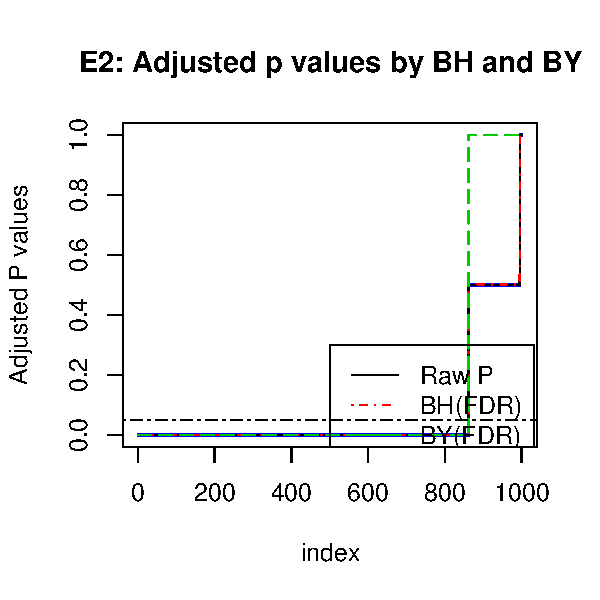
\includegraphics[width=0.8\textwidth]{IsoGene-IsoBHPlot.pdf}}
\caption{\em {The unadjusted (solid blue line), and the BH-FDR
(dotted and dashed red line) and BY-FDR (dashed green line) adjusted
$p$-values for $\bar{E}_{01}^2$.}} \label{IsoBHPlot}
\end{figure}



\section{Significance Analysis of Dose-response Microarray Data (SAM)}

In this package, we also implement the significance analysis of microarray (SAM) for testing
for the dose-response relationship under order restricted alternatives. The SAM procedure was proposed
by Tusher \textit{et al.}\ (2001) for finding differentially expressed genes by using permutations while controlling for
the FDR.

The main function for the SAM procedure is \texttt{IsoTestSAM()}. Within the main function, \texttt{Isofudge()}
calculates the fudge factor in the SAM test statistic, \texttt{IsoGenemSAM()} is used
to obtain the values of SAM test statistics, \texttt{Isoqqstat()} calculates the SAM test statistic
for the required number of permutations specified by users, \texttt{Isoallfdr()} obtains the delta table in the SAM procedure,
\texttt{Isoqval()} computes q-values of the SAM.  %And we can use \texttt{IsoSAMPlot}() to display outputs of the SAM.

The syntax of these function is as follows,

\begin{Schunk}
\begin{Sinput}
> Isofudge(x, y)
> IsoGenemSAM(x, y, fudge.factor)
> Isoqqstat(x, y, fudge = c(0, "pooled"), niter = 100)
> Isoallfdr(qqstat, ddelta, stat = c("E2", "Williams", "Marcus", 
+     "M", "ModifM"))
> Isoqval(delta, allfdr, qqstat, stat)
\end{Sinput}
\end{Schunk}

We use the same data as above to obtain the fudge factor of the SAM procedure for
the five test statistics by using function \texttt{Isofudge()}.

\begin{Schunk}
\begin{Sinput}
> fudge.factor <- Isofudge(x, exampleData)
\end{Sinput}
\end{Schunk}

The output of this function gives a vector of five fudge factors for each of the test statistics.

\begin{Schunk}
\begin{Sinput}
> fudge.factor
\end{Sinput}
\begin{Soutput}
[1] 0.07794229 0.16687744 0.10486056 0.19962253 0.12201373
\end{Soutput}
\end{Schunk}

Note that the fudge factor of the $\bar{E}_{01}^2$ is obtained based on the algorithm for F test
statistics given by Tusher \textit{et al.}\ (2001) and should be used with cautions. The performance of using
the fudge factor as compared to the $t$-type test statistics has not yet investigated in term of
power and control of the FDR. Therefore, it's advisable to use the fudge factor in the $t$-type test statistics.

\begin{Schunk}
\begin{Sinput}
> SAMtest.stat <- IsoGenemSAM(x, exampleData, fudge.factor)
\end{Sinput}
\end{Schunk}

The output of the function gives

\begin{Schunk}
\begin{Sinput}
> names(SAMtest.stat)
\end{Sinput}
\begin{Soutput}
[1] "E2"        "Williams"  "Marcus"    "M"         "ModM"      "direction"
\end{Soutput}
\end{Schunk}

The following codes produce the values of the five test statistics for the first ten genes,

\begin{Schunk}
\begin{Sinput}
> SAMtest.stat[[1]][1:10]
\end{Sinput}
\begin{Soutput}
        g1         g2         g3         g4         g5         g6         g7 
0.76307188 0.24474561 0.79981561 0.04428623 0.25513904 0.26372825 0.08792619 
        g8         g9        g10 
0.05322140 0.16347105 0.98418205 
\end{Soutput}
\begin{Sinput}
> SAMtest.stat[[2]][1:10]
\end{Sinput}
\begin{Soutput}
 [1]  2.524719216  0.568405925  2.795837275  0.335299641 -0.393142350
 [6] -0.477446410 -0.333583454 -0.006801912 -0.529556199  9.327805999
\end{Soutput}
\begin{Sinput}
> SAMtest.stat[[3]][1:10]
\end{Sinput}
\begin{Soutput}
 [1]  3.1845748  1.0392371  3.6000422  0.4121190 -1.0291185 -1.0024228
 [7] -0.5207607  0.4260847 -0.6845731 12.8347836
\end{Soutput}
\begin{Sinput}
> SAMtest.stat[[4]][1:10]
\end{Sinput}
\begin{Soutput}
 [1]  2.0885434  0.6862569  2.4788191  0.2999204 -0.5940818 -0.6202021
 [7] -0.3818276  0.2994731 -0.4229476  7.5100918
\end{Soutput}
\begin{Sinput}
> SAMtest.stat[[5]][1:10]
\end{Sinput}
\begin{Soutput}
 [1]  2.6588739  0.8578876  3.1369183  0.3561781 -0.7907050 -0.8276609
 [7] -0.4648386  0.3617761 -0.5797297 10.2222441
\end{Soutput}
\begin{Sinput}
> SAMtest.stat[[6]][1:10]
\end{Sinput}
\begin{Soutput}
 g1  g2  g3  g4  g5  g6  g7  g8  g9 g10 
"u" "u" "u" "u" "d" "d" "d" "u" "d" "u" 
\end{Soutput}
\end{Schunk}


To obtain the SAM test statistics for one of five test statistic values, for example, the modified M test,
with the required number of permutations specified by users and compute the
delta table in the SAM procedure, we can use function \texttt{Isoqqstat()} and \texttt{Isoallfdr()} as follows,

\begin{Schunk}
\begin{Sinput}
> qqstat <- Isoqqstat(x, exampleData, fudge = "pooled", niter = 2)
> dtable <- Isoallfdr(qqstat, , stat = "ModifM")
\end{Sinput}
\end{Schunk}

\begin{Schunk}
\begin{Sinput}
> dim(dtable)
\end{Sinput}
\begin{Soutput}
[1] 124   6
\end{Soutput}
\end{Schunk}
% latex table generated in R 2.7.2 by xtable 1.5-4 package
% Thu May 07 15:11:26 2009
\begin{table}[!h]
\begin{left}
\begin{tabular}{llllll}
 Ddelta & FalsePositive50\% & FalsePositive90\% & Called & FDR50\% & FDR90\% \\
 0.01 & 464.905 & 468.4274 & 946 & 0.4914 & 0.4952 \\
  0.11 & 391.608 & 392.4368 & 875 & 0.4476 & 0.4485 \\
  0.21 & 341.88 & 342.2944 & 831 & 0.4114 & 0.4119 \\
  0.31 & 295.001 & 298.109 & 780 & 0.3782 & 0.3822 \\
  . & . & . & . & . & . \\
  . & . & . & . & . & . \\
  . & . & . & . & . & . \\
  12.01 & 0 & 0 & 2 & 0 & 0 \\
  12.11 & 0 & 0 & 2 & 0 & 0 \\
  12.21 & 0 & 0 & 2 & 0 & 0 \\
  12.31 & 0 & 0 & 2 & 0 & 0 \\
  \end{tabular}
\end{left}
\end{table}

Note that in \texttt{Isoallfdr()}, ddelta is left blank, with default value taken
from the data, i.e., all the percentiles of the standard errors.
By fixing the 50\% FDR at 0.05, the corresponding delta value is 0.83
(marked in-between the dashed lines) as we obtain from the delta table above,
the number of differentially expressed genes are 872 with potential 42 genes as false positives.

%%% MAKE TABLE %%%%
\begin{Schunk}
\begin{Sinput}
> qval <- Isoqval(delta = 0.83, allfdr = dtable, qqstat = qqstat, 
+     stat = "ModifM")
> dim(qval[[1]])
\end{Sinput}
\begin{Soutput}
[1] 1000    3
\end{Soutput}
\end{Schunk}

% latex table generated in R 2.7.2 by xtable 1.5-4 package
% Thu May 07 15:11:26 2009
\begin{table}[!h]
\begin{left}
\begin{tabular}{rlll}
  & Row.names & t.stat & q.val \\
 g987 & 987 & -6.74228306204571 & 0 \\
  g409 & 409 & -6.71742170523205 & 0 \\
  g374 & 374 & -6.60269415492767 & 0 \\
  g229 & 229 & -5.56938272627751 & 0 \\
  g963 & 963 & -4.95269057984541 & 0 \\
  g962 & 962 & -4.81360570852988 & 0 \\
   & .. & .. & .. \\
  g514 & 514 & 7.04185921104539 & 0 \\
  g994 & 994 & 8.12042209576496 & 0 \\
  g190 & 190 & 10.1466161053291 & 0 \\
  g10 & 10 & 10.2222440760698 & 0 \\
  g148 & 148 & 14.2708293737359 & 0 \\
  g51 & 51 & 19.9115921617328 & 0 \\
  \end{tabular}
\end{left}
\end{table}
\begin{Schunk}
\begin{Sinput}
> dim(qval[[2]])
\end{Sinput}
\begin{Soutput}
[1] 231   3
\end{Soutput}
\end{Schunk}


% latex table generated in R 2.7.2 by xtable 1.5-4 package
% Thu May 07 15:11:26 2009
\begin{table}[!h]
\begin{left}
\begin{tabular}{rlll}
  & Row.names & t.stat & q.val \\
 g987 & 987 & -6.74228306204571 & 0 \\
  g409 & 409 & -6.71742170523205 & 0 \\
  g374 & 374 & -6.60269415492767 & 0 \\
  g229 & 229 & -5.56938272627751 & 0 \\
  g963 & 963 & -4.95269057984541 & 0 \\
  g962 & 962 & -4.81360570852988 & 0 \\
   & ... & ... & ... \\
  g514 & 514 & 7.04185921104539 & 0 \\
  g994 & 994 & 8.12042209576496 & 0 \\
  g190 & 190 & 10.1466161053291 & 0 \\
  g10 & 10 & 10.2222440760698 & 0 \\
  g148 & 148 & 14.2708293737359 & 0 \\
  g51 & 51 & 19.9115921617328 & 0 \\
  \end{tabular}
\end{left}
\end{table}
By specifying the desired delta value, delta table, and the user-defined test statistic in function \texttt{Isoqval()}, we can obtain
the q value of each gene from the SAM procedure. The first object of the output is the list of q values for
all the genes, ranking from the smallest test statistic value to the largest; while the second object is the list of q values
for the 872 differentially expressed genes, ranking from the smallest test statistic value to the largest. The first column of the output matrices is the row number of genes in
the data set, the second column is the observed modified M test statistic value, and the last column is the q value of the
SAM procedure for both objects.

Alternatively, we can use function \texttt{IsoTestSAM()} to summarize all the steps above and give results of a list of significant findings, which is the same second output of function \texttt{Isoqval()}.

\begin{Schunk}
\begin{Sinput}
> IsoTestSAM(x, y = data, fudge = c(0, "pooled"), niter = 100, 
+     FDR = 0.05, stat = c("E2", "Williams", "Marcus", "M", "ModifM"))
\end{Sinput}
\end{Schunk}

Specifying the same options as above in this function, we can obtain the list of significant genes as follows: the first column is the Probe.ID, the second column is the corresponding row numbers of the genes in the data set, the third column is the observed modified M SAM test statistics, the fourth column is the $q$ values of genes by using the SAM procedure. The last two columns gives additional information by calculating the $p$ values based on the SAM permutation matrix and adjusting these $p$ values using the BH-FDR procedure.

%%% MAKE TABLE %%%%

\begin{Schunk}
\begin{Sinput}
> IsoSAM.obj <- IsoTestSAM(x, y = exampleData, fudge = "pooled", 
+     niter = 2, FDR = 0.05, stat = "ModifM")
> dim(IsoSAM.obj)
\end{Sinput}
\begin{Soutput}
[1] 247   6
\end{Soutput}
\end{Schunk}

% latex table generated in R 2.7.2 by xtable 1.5-4 package
% Thu May 07 15:11:33 2009
\begin{table}[!h]
\begin{left}
\begin{tabular}{llllll}
 Probe.ID & row.number & stat.val & qvalue & pvalue & adj.pvalue \\
 g987 & 987 & -6.74228306204571 & 0 & 0 & 0 \\
  g409 & 409 & -6.71742170523205 & 0 & 0 & 0 \\
  g374 & 374 & -6.60269415492767 & 0 & 0 & 0 \\
  g229 & 229 & -5.56938272627751 & 0 & 0 & 0 \\
  g963 & 963 & -4.95269057984541 & 0 & 0 & 0 \\
  g962 & 962 & -4.81360570852988 & 0 & 0 & 0 \\
   & . & . & . & . & . \\
   & . & . & . & . & . \\
   & . & . & . & . & . \\
  g514 & 514 & 7.04185921104539 & 0 & 0 & 0 \\
  g994 & 994 & 8.12042209576496 & 0 & 0 & 0 \\
  g190 & 190 & 10.1466161053291 & 0 & 0 & 0 \\
  g10 & 10 & 10.2222440760698 & 0 & 0 & 0 \\
  g148 & 148 & 14.2708293737359 & 0 & 0 & 0 \\
  g51 & 51 & 19.9115921617328 & 0 & 0 & 0 \\
  \end{tabular}
\end{left}
\end{table}

Finally, the graphic output of the SAM procedure can be produced using function \texttt{IsoSAMPlot()}.

\begin{Schunk}
\begin{Sinput}
> IsoSAMPlot(qqstat, allfdr, FDR = 0.05, stat = c("E2", "Williams", 
+     "Marcus", "M", "ModifM"))
\end{Sinput}
\end{Schunk}

This function requires the use of output from \texttt{Isoqqstat()} and \texttt{Isoallfdr()}, given a user-defined test statistic
and the FDR level to control. We still take the modified M test statistic for example, at the FDR of 0.05. There are four plots
yielded from the SAM procedure. Panel $a$ shows the FDR (either 50\% or 90\% (more stringent)) vs. $\Delta$, from which, user can choose the delta value with
the corresponding desired FDR. Panel $b$ shows the number of significant genes vs. $\Delta$, and panel $c$ shows the number of false positives (either 50\% or 90\%) vs. $\Delta$. Finally panel $d$ shows the observed vs. the expected (obtained from permutations) test statistics, in which the red dots are those genes called differentially expressed.

\begin{Schunk}
\begin{Sinput}
> IsoSAMPlot(qqstat = qqstat, allfdr = dtable, FDR = 0.05, stat = "ModifM")
\end{Sinput}
\end{Schunk}

 
  
\clearpage
\newpage


\begin{figure}[!h]
\centering
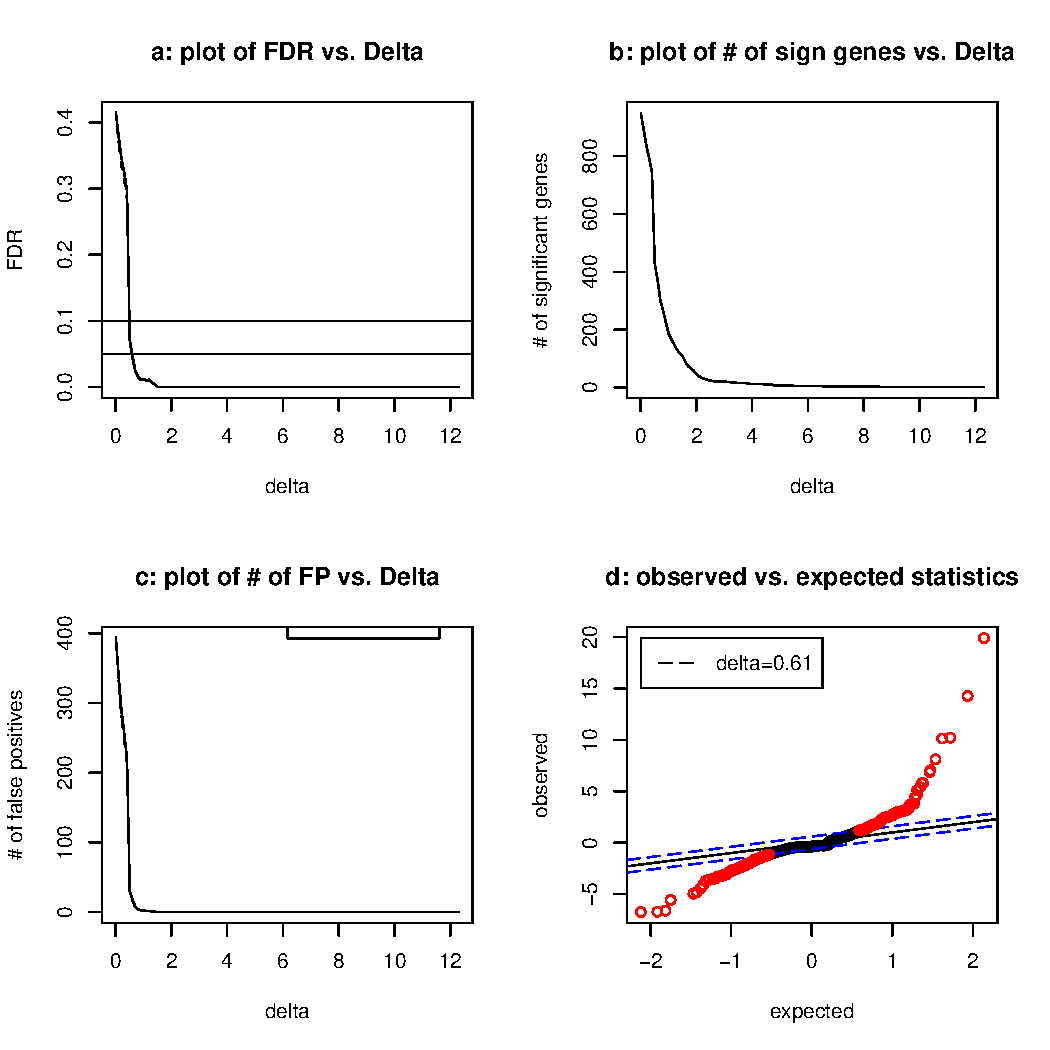
\includegraphics[width=1\textwidth]{IsoGene-IsoSAMPlotOutput.pdf}
\caption{\em {The SAM plots: a.Plot of the FDR vs. delta; b. Plot of number of significant genes vs. delta; c. Plot of
number of false positives vs. delta; d. Plot of observed vs. expected test statistics.}} 
\label{IsoBHPlot}
\end{figure}


\clearpage
\newpage


\section*{References}


\begin{list}{}{\setlength{\leftmargin}{.3in}\setlength{\itemindent}{-.2in}}

\item Agresti, A. (1997) \textit{Statistical Methods for the
Social Sciences}, Finlay.

\item Barlow, R.E., Bartholomew, D.J.,
Bremner, M.J. and Brunk, H.D. (1972) \textit{Statistical inference
under order restriction}, New York: Wiley.

\item Bartholomew, D.J. (1961) Ordered
tests in the analysis of variance, \textit{Biometrika}, \textbf{48},
325--332.%

\item Benjamini, Y. and Hochberg, Y.
(1995) Controlling the false discovery rate: a practical and
powerful approach to multiple testing. \textit{Journal of Royal
Statistical Soceity, Biostatistics}, \textbf{57}, 289--300.%


\item Benjamini, Y. and Yekutieli,
D. (2001) The control of the false discovery rate in multiple
testing under dependency. \textit{Annal of Statistics},
\textbf{29(4)}, 1165--1188.%


\item
Benjamini, Y. and Yekutieli, D. (2005) False Discovery
Rate-Adjusted Multiple Confidence Intervals for Selected Parameters.
{\em Journal of the American Statistical Association}, \textbf{100}, 71--81.%


\item Chuang-Stein, C. and Agresti, A. (1997) Tutorial in biostatistics:
A review of tests for detecting a monotone dose-response
relationship with ordinal response data, \textit{Statistics in
Medicine}, \textbf{16}, 2599--2618.%


\item Ge, Y., Dudoit, S. and Speed, P.T.
(2003) Resampling based multiple testing for microarray data
analysis,  \textit{technical report}, \textbf{633}, University of
Berkeley.%

\item Hu, J., Kapoor, M., Zhang, W.,
Hamilton, S.R. and Coombes, K.R. (2005) Analysis of dose response
effects on gene expression data with comparison of two microarray
platforms, \textit{Bioinformatics}, \textbf{21(17)}, 3524--3529.%

\item Lin, D., Shkedy, Z., Yekutieli, D., Burzykowki,
T., G\"{o}hlmann, H.W.H., De Bondt, A., Perera, T., Geerts, T.,
Bijnens, L. (2007a) Testing for trend in dose-response microarray
experiments: comparison of several testing procedures, multiplicity,
and resampling-based inference. \textit{Statistical Application in
Genetics and Molecular Biology}, \textbf{6(1)}, article 26.%

\item Lin, D., Shkedy, Z., Burzykowki, R., Ion,
T., G\"{o}hlmann, H.W.H., De Bondt, A., Perera, T., Geerts, T.,
Bijnens, L. (2008) An investigation on performance of Significance
Analysis of Microarray (SAM) for the comparisons of several
treatments with one control in the presence of small variance genes.
\textit{Biometrical Journal}, Multiple Comparison Problem, Special Issue,
\textbf{50(5)}, 801--823.%



\item Marcus, R. (1976) The powers of some tests of
the quality of normal means against an ordered alternative,
\textit{Biometrika}, \textbf{63}, 177--83.%

\item Reiner, A., Yekutieli, D. and
Benjamini, Y. (2003) Identifying differentially expressed genes
using false discovery rate controlling procedures.
\textit{Bioinformatics}, \textbf{19(3)}, 368--375.%

\item Robertson, T., Wright, F.T. and Dykstra, R.L. (1988) \textit{ Order restricted statistical inference}, Wiley.%



item Ruberg, S.J. (1995a) Dose response studies. I. Some design
considerations. \textit{Journal of Biopharmaceutical Statistics},
\textbf{5(1)}, 1--14.%

\item Ruberg, S.J. (1995b) Dose response studies. II. Analysis and
interpretation. \textit{Journal of Biopharmaceutical Statistics},
\textbf{5(1)}, 15--42.%

\item Tusher, V.G., Tibshirani, R. and
Chu, G. (2001) Significance analysis of microarrys applied to the
ionizing radiation response, \textit{Proceedings of the National
Academy of Sciences}, \textbf{98} , 5116--5121.%


\item Williams, D.A. (1971) A test for differences between treatment
means when several dose levels are compared with a zero dose
control, \textit{Biometrics}, \textbf{27}, 103--117.%

\item Williams, D.A. (1972) The comparision of several dose levels
with a zero dose control, \textit{Biometrics}, \textbf{28},
519--531.%


\end{list}















\newpage\thispagestyle{empty} $^{}$
\newpage
%\part{Discussion}
%\include{Discussion}



%\appendix
%\include{AppenA}

%\newpage\thispagestyle{empty} $^{}$
%\newpage
%\include{AppenB}


%\newpage\thispagestyle{empty} $^{}$
%\newpage
%\include{doctnl0a}



\end{document}


%\newpage\thispagestyle{empty}
%\marksam{Samenvatting} \marksection{Samenvatting}

%\newpage\thispagestyle{empty}


